%%\documentclass[sn-nature]{sn-jnl}% Style for submissions to Nature Portfolio journals
%%\documentclass[sn-basic]{sn-jnl}% Basic Springer Nature Reference Style/Chemistry Reference Style
\documentclass[sn-mathphys,Numbered]{sn-jnl}
\usepackage{graphicx}%
\usepackage{multirow}%
\usepackage{amsmath,amssymb,amsfonts}%
\usepackage{amsthm}%
\usepackage{mathrsfs}%
\usepackage[title]{appendix}%
\usepackage{xcolor}%
\usepackage{textcomp}%
\usepackage{manyfoot}%
\usepackage{booktabs}%
\usepackage{algorithm}%
\usepackage{algorithmicx}%
\usepackage{algpseudocode}%
\usepackage{listings}%
\usepackage[normalem]{ulem}
\usepackage{comment}

% Make Orcid icon
\newcommand{\orcidicon}{
\includegraphics[width=0.32cm]{orcid.pdf}}
\newcommand{\orc}[1]{\href{https://orcid.org/#1}{\orcidicon}}

% Author Orcid ID: Define per author
\newcommand{\orcA}{0000-0001-8217-1484}
\newcommand{\orcB}{0000-0001-5038-8427}
\newcommand{\orcC}{0000-0001-5474-2649}
\newcommand{\orcD}{0000-0003-2704-6474}
\newcommand{\orcE}{0000-0002-2289-4856}

% List of useful macros
\newcommand{\wt}[1]{\widetilde{#1}}
\newcommand{\req}[1]{Eq.~(\ref{#1})}
\newcommand{\rf}[1]{Fig.~{\ref{#1}}}
\newcommand{\rt}[1]{Table~{\ref{#1}}}
\newcommand{\rsec}[1]{Sec.~{\ref{#1}}}
\newcommand*{\TeV}{\text{ TeV}}
\newcommand*{\GeV}{\text{ GeV}}
\newcommand*{\MeV}{\text{ MeV}}
\newcommand*{\keV}{\text{ keV}}
\newcommand*{\eV}{\text{ eV}}
\newcommand*{\meV}{\text{ meV}}
\DeclareMathOperator{\sgn}{sgn}

% Useful macros for annotation
\newcommand*{\xred}{\color{red}}
\newcommand*{\xblue}{\color{blue}}
\newcommand*{\xgreen}{\color{green}}
\newcommand*{\xmagenta}{\color{magenta}}
\newcommand{\rev}[1]{{\color{blue}#1}}
\newcommand*{\rcite}{{\xred (Citation?)}}

%\theoremstyle{thmstyleone}%
\newtheorem{theorem}{Theorem}
\newtheorem{corollary}[theorem]{Corollary} 
\newtheorem{lemma}[theorem]{Lemma} 
%\theoremstyle{thmstyletwo}%
%\newtheorem{example}{Example}%
\newtheorem{remark}{Remark}
%\theoremstyle{thmstylethree}%
%\newtheorem{definition}{Definition}%

\raggedbottom
\begin{document}

%\title[Article Title]{Cold Ideal Fermi Gas}
\title[Article Title]%{Zero and finite temperature  components of\newline the Fermi quantum gas}
{Asymptotic Expansion Near Fermi Surface}
%%=============================================================%%
%% Prefix	-> \pfx{Dr}
%% GivenName	-> \fnm{Joergen W.}
%% Particle	-> \spfx{van der} -> surname prefix
%% FamilyName	-> \sur{Ploeg}
%% Suffix	-> \sfx{IV}
%% NatureName	-> \tanm{Poet Laureate} -> Title after name
%% Degrees	-> \dgr{MSc, PhD}
%% \author*[1,2]{\pfx{Dr} \fnm{Joergen W.} \spfx{van der} \sur{Ploeg} \sfx{IV} \tanm{Poet Laureate} 
%%                 \dgr{MSc, PhD}}\email{iauthor@gmail.com}
%%=============================================================%%
 
\author[1]{\hspace*{1.5cm}\fnm{Cheng Tao} \sur{Yang\orc{\orcB}}}
\author[1]{\fnm{Jeremiah} \sur{Birrell\orc{\orcE}}}
\author[1,2]{\fnm{Martin} \sur{Formanek\orc{\orcD}}}
\author[1]{\fnm{Andrew} \sur{Steinmetz\orc{\orcC}}} 
\author[1]{\fnm{Johann} \sur{Rafelski\orc{\orcA}}}

%\email{iiiauthor@gmail.com}
%\equalcont{These authors contributed equally to this work.}

\affil[1]{\orgdiv{Department of Physics}, \orgname{The University of Arizona}, \city{\newline Tucson}, \state{Arizona}, \postcode{85721}, \country{USA}}

\affil[2]{\orgdiv{ELI Beamlines Facility}, \orgname{The Extreme Light Infrastructure ERIC}, \orgaddress{ \postcode{\newline 252 41}  \city{Doln\'{i} B\v{r}e\v{z}any}, \country{Czech Republic}}}

\abstract{We present a novel mathematical tool allowing to separate the zero and finite temperature phenomena in ideal Fermi gases. To achieve this  we decompose the Fermi distribution into three components. We prove that the singular (step) functions properly add up to the finite temperature smooth Fermi shape. As an example we consider briefly a semi relativistic-electron density where with high chemical potential ($\mu>m$) at low temperature $T<<m$. \xblue{Point out that the Sommerfild doesn't work in certain domain, and our asymptotic expansion work in this domain}}

% ANDREW's note: We present a novel mathematical tool allowing the separation of the finite and zero temperature phenomena in fermi gassses. To achieve this, we provide a novel form of the Fermi distribution 

\date{January 2024, To be published in International Journal of Theoretical Physics}
\keywords{Fermi distribution, Low temperature}

%%\pacs[JEL Classification]{D8, H51}
%%\pacs[MSC Classification]{35A01, 65L10, 65L12, 65L20, 65L70}

\maketitle

%%%%%%%%%%%%%%%%%%%%%%%%%%%%%%%%%%%%%%%
\section{Introduction}
\label{sec1}
%%%%%%%%%%%%%%%%%%%%%%%%%%%%%%%%%%%%%%%

% Andrew's note (2/26/2024): Can the 1st derivative delta function problem present in other mathematical examples of derivatives of distributions? If so, then this clarifies the issue and separates it entirely from the complexity of the FD distribution. Suggested mathematical example to try: f(x) = FD(x) - Heaviside(x). Hmm...

% Second solution idea: Redo the derivative derivation however treating all singular functions as couched within an integration. E.g. no naked distributions! Do then physical measurable quantities suffer from this inconsistancy? I suspect not. Therefore there is no problem.

% Andrew's Note (4/15/2024): Emphasize motivation via the low temperature limit.

The zero temperature limit of Fermi-Dirac (FD) distribution involves a transition from a smooth functional form to a singular Heaviside step function. Such singular limit  $T\to 0$ therefore cannot be analytical. For this reason a study of finite temperature effects in dense low temperature FD quantum gasses poses a mathematical challenge and can miss key physical features. To remedy this situation we introduce here a novel reformulation which allows exact separation of the finite temperature behavior from the singular zero temperature limit. This means that we will be replacing the smooth FD distribution by the sum of three singular functions
$$
\boxed{\frac{1}{e^{x} +1}=\Theta(-x)+\frac{1}{2}e^{-|x|}\left[\sgn(x)+\tanh(x/2)\right]}
$$
one being the $T=0$ limit, the other two describing the finite temperature residual. In the following we illuminate the advantages offered by this decomposition.

The most interesting physics of FD gasses occurs at finite temperatures~\cite{bludman1977equation,Elze:1980er} which necessitates a mathematical tool which captures the finite temperature behavior of the FD distribution. We provide a novel form of FD distribution that manifestly separates the zero and finite temperature contributions so that the finite temperature correction can be studied on its own. We also tackle the case of the semi-relativistic electron gas to demonstrate the usefulness of this new method. The asymptotic limit of integrals of the FD distribution~\cite{dingle1957fermi,dingle1973asymptotic} is of great interest to physicists studying statistical quantum systems~\cite{10.1063/1.1350634,10.1142/S021827180701002X,10.1063/1.1665160,FUKUSHIMA2014417,GIL2022126618,GIL2023108563} and behavior around the Fermi surface~\cite{kim2008notes,PhysRevB.103.205154}. Other use cases would be for compact astrophysical systems (white dwarfs, neutron stars, quark stars)~\cite{Kaspi:2017fwg,Ferrer:2019xlr,Ferrer:2023pgq}, Early Universe phenomenology~\cite{Rafelski:2021aey,Rafelski:2023emw,Grayson:2023flr,Steinmetz:2023nsc}, quark-gluon plasmas (QGP)~\cite{Letessier:2002ony,Rafelski:2020ajx,Yang:2021bko}, and in any situation when finite temperature Fermi effects are important. This is of special interest to the regime of neutrino cosmology where the neutrinos are very cold with a small chemical potential mirroring the baryon asymmetry in the universe~\cite{Birrell:2013gpa,Birrell:2012gg}.

%Before we introduce the novel form in \rsec{NewFermi}, we will briefly recall the standard picture of the FD distribution. 

The illustration of the problem is presented in \rf{Electron_001}: In the zero temperature limit $T\to0$, the FD distribution reduces to a step function where a state $E_{i}$ is either filled or empty. For given chemical potential $\mu(T)$, we have
\begin{align}
\label{f_old}
f_\mathrm{FD}[E_{i},\mu(T),T]=\left[\exp\left(\frac{E_{i}-\mu}{T}\right)+1\right]^{-1}\,,\quad
\lim_{T\to0}f_\mathrm{FD}=\left\{
\begin{array}{c}
1,\quad\mathrm{for}\quad{E_{i}}<\mu\\
0,\quad\mathrm{for}\quad{E_{i}}>\mu
\end{array}
\right.\,.
\end{align}
The energy of the last filled state is called the Fermi energy and is denoted by $E_F$. The Fermi energy is also the value of the chemical potential at zero temperature $T=0$, \emph{i.e.} $E_F\equiv\mu(T = 0)$.
%%%%%%%%%%%%%%%%%%%%%%%%%%%%%%%%%%%%%%%
\begin{figure}[ht]
\centering
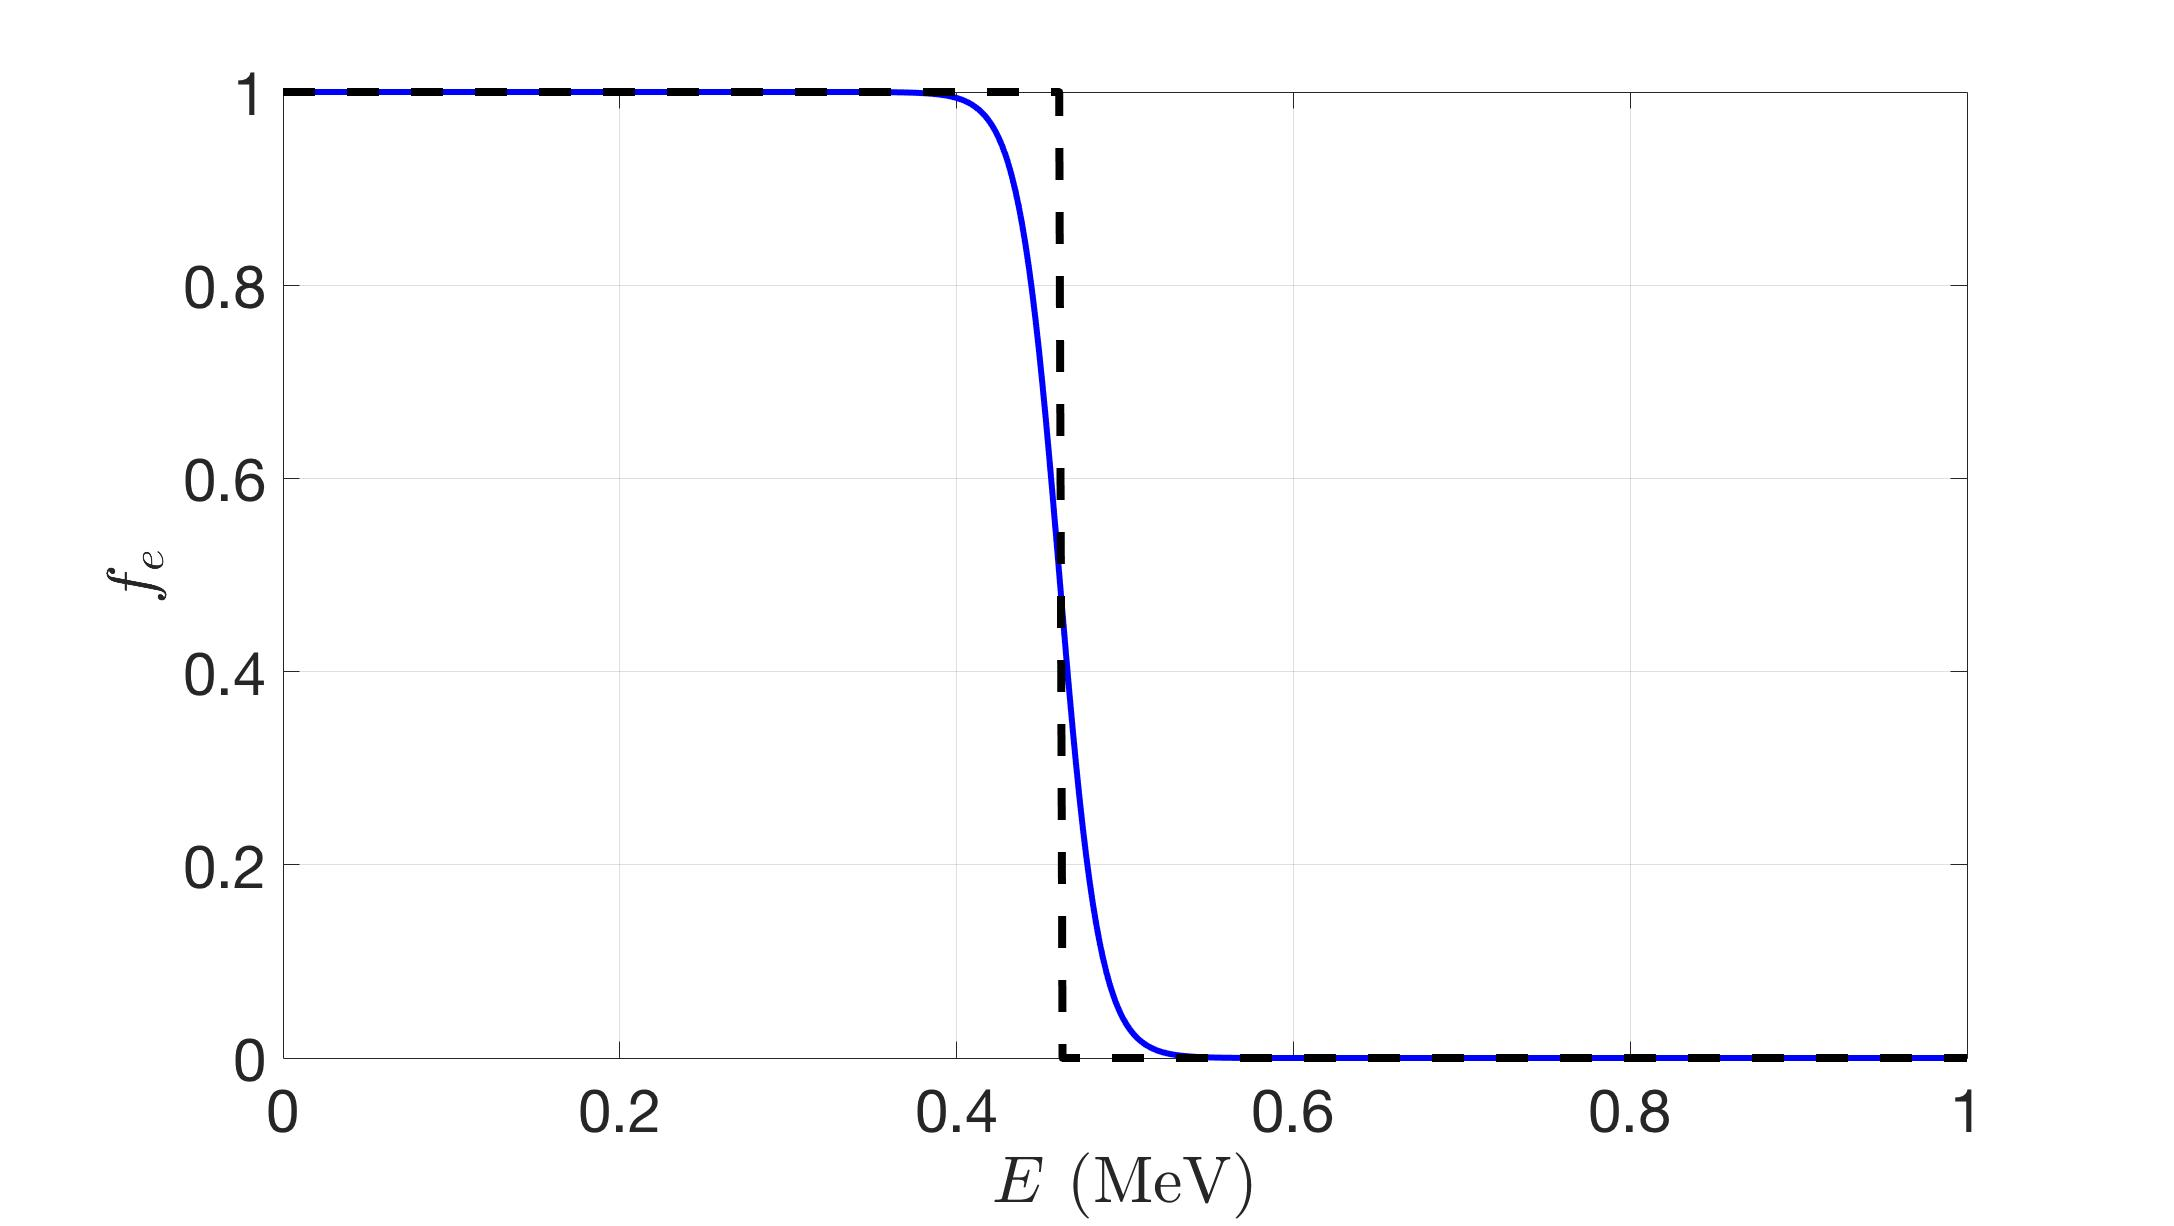
\includegraphics[width=0.9\textwidth]{./plot/Electron_distribution001}
\caption{The FD distribution is plotted (solid blue line) as a function of energy with parameters $T=0.012\MeV$ and $\mu=0.461\MeV$. The zero temperature distribution is plotted as the dashed black line.}
\label{Electron_001}
\end{figure}
%%%%%%%%%%%%%%%%%%%%%%%%%%%%%%%%%%%%%%%

In \rf{Electron_001} the solid line shows Fermi distribution as a function of energy for temperature $T=0.012\MeV$, chemical potential $\mu=0.461\MeV$, and electron mass $m=0.511\MeV$. Dashed line is the corresponding $T=0$ limit.  This demonstrates the textbook behavior that for finite temperature $T > 0$, even states above the chemical potential $\mu$ can be occupied at the expense of states below $\mu$. As the temperature increases, the distribution becomes broader as a wide range of states become thermally populated.

Our objective is to describe the difference between these two distributions in a format allowing to evaluate and study in semi-analytical way the finite temperature effects occuring near to the Fermi surface.

{\bf New points to incorporate into abstract/intro/conclusions}
\begin{enumerate}
\item The decomposition guides the asymptotic analysis of $\langle G\rangle_T-\langle G\rangle_0$ by naturally reorganizing the integrand into a difference of integrals with exponentially decaying integrands. This allows us to utilize asymptotic analysis techniques to   extract  leading and subleading order behavior as $T\to 0$. {(\color{blue} Incorporate into conclusion)}
\item The finite temperature contribution is naively written as a difference of integrals, with the leading order contribution in $T$ of the former canceling that of the latter.  This leads to instability when attempting to compute $\langle G\rangle_T-\langle G\rangle_0$ via numerical integration for small $T$.  This issue is eliminated when using the asymptotic expansion derived below, where we are able to account for this exact cancellation analytically. ({\color{blue} Incorporate into conclusion)}
\item The assumptions on $G(p)$ are quite modest, only requiring smoothness and polynomial growth bounds on $G$ and it's derivatives as $p\to \infty$.  The latter is only slightly more restrictive than simply assuming integrability.  These assumptions hold, for instance, in the case of ...({\color{blue} Incorporate into conclusion)}
\item The Sommerfeld expansion is asymptotic in nature (cite LL book, including footnote), meaning that adding further terms does not necessarily reduce the error at fixed values of $T$ and $\mu$.  This is particularly relevant when $\mu-m$ is small, a regime that the classical Sommerfeld expansion was not designed for.  When dealing with multiple scales, here $T$ and $\mu-m$, one generally requires specialized asymptotic expansions that are adapted to regime under consideration. ({\color{blue} Incorporate into Fig.3 and related content})
\end{enumerate}


 


\subsection{Summary of Results}
In this work we derive and contrast expansions in the following regimes which, to the best of the authors' knowledge, are new:
\begin{enumerate}
\item High-temperature Sommerfeld: $\mu\gg T\gg m$; see  Section \ref{Section:HighTempSommerfeld} and Theorem \ref{thm:high_T_Sommerfeld}.
\item ??descriptive name for this regime??: $T\ll \mu-m\ll m$; see Section \ref{sec:asymp_T_0_faster} and Theorem \ref{thms:T_decay_faster}.
\item ??descriptive name for this regime??: $\mu-m\ll T\ll m$; see Section \ref{sec:asympt_Delta_mu_order_T} and Theorem \ref{thm:mu_zero_faster}
\end{enumerate}
First, we prove that the classical Sommerfeld expansion, which applies to the regime $T\ll m$ with $\mu-m$ not small, also applies to the high-temperature regime $\mu\gg T\gg m$ under appropriate assumptions.  In this derivation we utilize a novel decomposition of the FD distribution into finite and zero temperature components, which we find convenient for guiding this and other derivations. Next we demonstrate that the Sommerfeld expansion can fail completely when applied to certain regimes where $\mu-m$ and $T$ are both small small; see  the example in Figure \ref{lnZ_Ratio_fig} below. Accurate results in the regime where both $\Delta\mu\ll T\ll m$ ($\Delta\mu\equiv \mu-m$)  requires the use of the new expansion presented in Theorem \ref{thm:mu_zero_faster}. In addition, the application of the classical Sommerfeld expansion to the case where $T\ll\Delta\mu\ll m$ requires care, as the coefficients in the expansion become singular in general;  in Theorem \ref{thms:T_decay_faster} we provide a formula that  resolves those singularities so as to avoid such numerical difficulties and obtain an expansion up to a specified order. We compare the domain of validity of the Sommerfeld expansion and the expansion from  Theorem \ref{thm:mu_zero_faster} in Figure \ref{fig:Thm3_vs_Sommerfeld_regions}. 


\begin{figure}
\centering
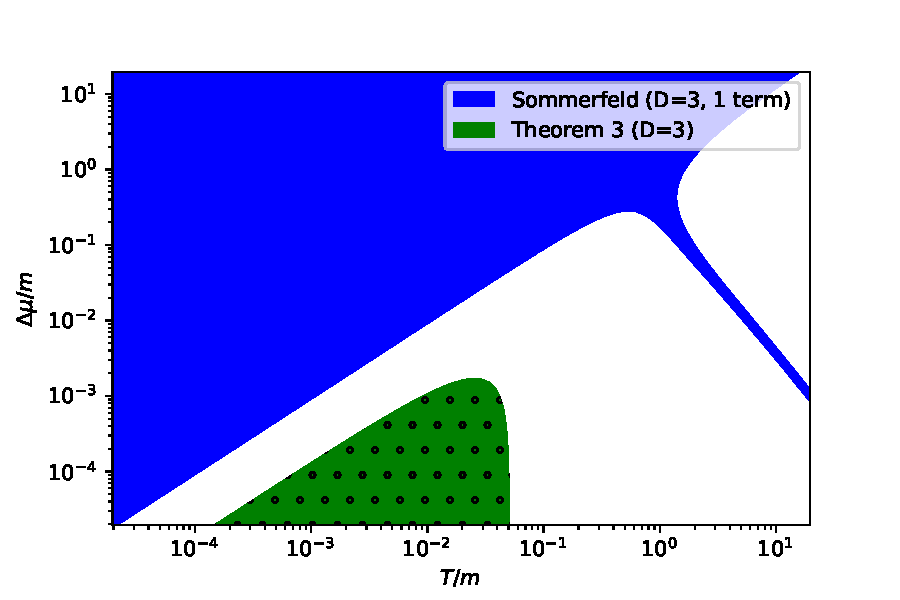
\includegraphics[width=0.49\textwidth]{./plot/Sommerfeld_vs_Thm3_regions_D3_1_term.pdf}
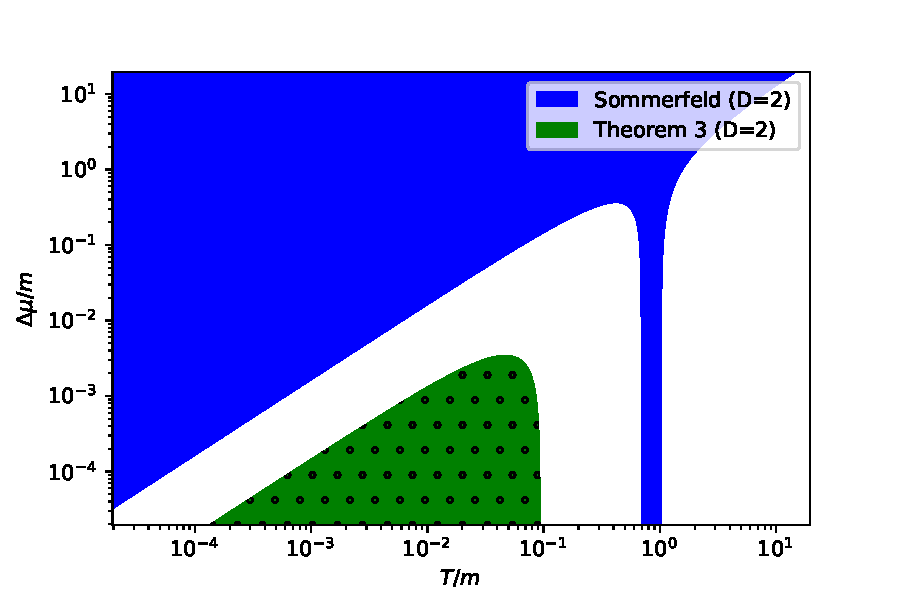
\includegraphics[width=0.49\textwidth]{./plot/Sommerfeld_vs_Thm3_regions_D2_1_term.pdf}
\caption{Domains of validity in $(T/m,\Delta\mu/m)$-space ($\Delta\mu\equiv\mu-m$) of the Sommerfeld expansion (solid blue) and the new expansion from Theorem \ref{thm:mu_zero_faster} (dotted green),  where validity is defined as the computation of $\langle G\rangle_T$ having relative error  less that $10\%$ for the choice  $G(p)=1$.  Our  expansion from Theorem \ref{thm:mu_zero_faster} applies when $\Delta\mu\ll T\ll m$, and its region of validity is larger in dimension $D=2$ than in $D=3$.  Note that in addition to the well-known low temperature regime, there is also a high-temperature regime ($\mu\gg T\gg m$) where the Sommerfeld expansion is valid; we  prove this in Theorem \ref{thm:high_T_Sommerfeld} below. }\label{fig:Thm3_vs_Sommerfeld_regions}
\end{figure}





%%%%%%%%%%%%%%%%%%%%%%%%%%%%%%%%%%%%%%%
\section{Zero and finite temperature Fermi-Dirac distributions}
\label{NewFermi}
%%%%%%%%%%%%%%%%%%%%%%%%%%%%%%%%%%%%%%%
\subsection{A novel form of Fermi-Dirac distribution}
\label{Novel}
%%%%%%%%%%%%%%%%%%%%%%%%%%%%%%%%%%%%%%%
Our interest and motivations in studying the Fermi-Dirac distribution was to perform cosmological computations involving both high and low temperature physics. In doing so, we have identified the following novel way to write FD distribution as three terms which separates out the zero temperature portion from the finite temperature contributions as 
\begin{align}
\label{NFF1}
\begin{split}
f_\mathrm{FD}(x)
&=\frac{1}{e^{x}+1}\,,\quad
x\equiv\frac{E-\mu}{T}\,,\\
\frac{1}{e^{x} +1}&=\Theta(-x)+\frac{1}{2}e^{-|x|}\left[\sgn(x)+\tanh(x/2)\right]
\,,
\end{split}
\end{align}
\begin{align}
\label{NFF2}
\Theta(x)=\left\{
\begin{array}{r}
1,\quad\mathrm{for}\quad{x}>0\\
%1/2,\quad\mathrm{for}\quad{x}=0\\
0,\quad\mathrm{for}\quad{x}<0
\end{array}\right.\,,\qquad
\sgn(x)=\left\{
\begin{array}{r}
+1,\quad\mathrm{for}\quad{x}>0\\
%0,\quad\mathrm{for}\quad{x}=0\\
-1,\quad\mathrm{for}\quad{x}<0\\
\end{array}\right.\,,
\end{align}
where $\Theta(x)$ is the Heaviside step function and $\sgn(x)$ is the sign function and the equality is in the sense of distributions. In particular the values at $x=0$ are convention-dependent and do not affect our results. The first term $\Theta(-x)$ in \req{NFF1} represents the zero temperature portion of the FD distribution while the finite temperature terms are weighted by a decaying exponential function. The immediate benefit of this form is that numerical evaluations will naturally center around the Fermi surface of the system with finite temperature contributions exponentially suppressed. In the following section, we will show that both sides are truly equivalent.

%%%%%%%%%%%%%%%%%%%%%%%%%%%%%%%%%%%%%%%
\subsection{Mathematical proof}
\label{Proof}
%%%%%%%%%%%%%%%%%%%%%%%%%%%%%%%%%%%%%%%
To show the equivalency between the two distinct forms of the FD, we look at the three relevant regions of $x>0$, the origin $x=0$, and $x<0$. For $x>0$, \req{NFF1} evaluates as
\begin{equation}\label{eq:xpos}
    f_\mathrm{FD}(x>0) = 0 + \frac{1}{2}e^{-x}[1+\tanh(x/2)] = (e^x + 1)^{-1}\,.
\end{equation}
This can be seen by using the hyperbolic formula $\tanh(x/2)=(e^x-1)/(e^x+1)$. In a similar manner, the $x<0$ region evaluates as
\begin{equation}\label{eq:xneg}
    f_\mathrm{FD}(x<0) = 1 + \frac{1}{2}e^{x}[-1 + \tanh(x/2)] = (e^x + 1)^{-1}\,.
\end{equation}
As we are considering the expressions in the sense of distributions, this completes the proof.  The values at $x=0$ are convention-dependent and irrelevant for our purposes, as the point $x=0$ is a set of measure zero with respect to integration.

\begin{comment}
special care should be taken in evaluation of the origin. It can be shown that the left $x=0^{-}$ and right $x=0^{+}$ limits are equal via
\begin{align}
    \lim_{x\rightarrow 0^+} f_\mathrm{FD}(x) &= 0 + \frac{1}{2}(1 + 0) = \frac{1}{2}\,,\\
    \lim_{x\rightarrow 0^-} f_\mathrm{FD}(x) &= 1 + \frac{1}{2}(-1 + 0) = \frac{1}{2}\,,
\end{align}
which means that the limit of our expression at the origin $x=0$ exists and is equal to the value of the function in \req{f_old} at $x = 0$. With the definitions of the step function $\Theta(x)$ and sign function $\sgn(x)$ in \req{NFF2}, the limits for $x\rightarrow0^{\pm}$ are equal to the value of our function at the origin. Therefore, for all real $x\in\mathbb{R}$, our expression matches the original FD distribution \req{f_old}.
\end{comment}

\begin{comment}
Lastly, we check that the properties of the first derivative of \req{NFF1} are in agreement with the usual FD distribution. We write the first derivative of the singular distributions as 
\begin{align}
\label{NFF1b}
\frac{d}{dx}\Theta(-x)&=-\delta(x)\,,\qquad 
\frac{d}{dE}\Theta(-x)=-\frac{1}{T}\delta(x)\,,\\
\frac{d}{dx}\sgn(x)&=2\delta(x)\,,\,\,\quad 
\frac{d}{dE}\sgn(x)=\frac{2}{T}\delta(x)\,,
\end{align}
both without and with units and where $\delta(x)$ is the Dirac $\delta$-function. \rev{The first derivative of the original FD distribution is
\begin{equation}\label{eq:ffdder}
    \frac{d}{dE} f_{FD}(x) = \frac{1}{T} \frac{-1}{4\cosh^2 \frac{x}{2}}
\end{equation}
which goes in the $T \rightarrow 0^+$ limit to delta function (DOES IT REALLY? NORMALLY $\delta$ is limit of 1/cosh). Using
\begin{equation}
    \frac{d|x|}{dE} = \frac{d\text{sgn}(x)x}{dE} = \frac{1}{T}\text{sgn}(x) + \frac{2}{T}x\delta(x)
\end{equation}
we can evaluate the derivative of the novel form as 
\begin{equation}
    \begin{split}
    T \frac{d}{dE}f_N(x) &= -\delta(x) - \frac{1}{2}e^{-|x|}[\text{sgn}(x) + 2x\delta(x)]\text{sgn}(x) + e^{-|x|}\delta(x)\\
    &- \frac{1}{2}e^{-|x|}[\text{sgn}(x) + 2 x \delta(x)]\tanh\frac{x}{2} + \frac{1}{4}\frac{e^{-|x|}}{\cosh^2\frac{x}{2}}
    \end{split}
\end{equation}
It is quite straightforward to show that for $x > 0$ or $x<0$ this expression matches Eq. (\ref{eq:ffdder}) as it should because outside $x=0$ we don't expect any issues. For $x\neq 0$ we have
\begin{equation}
    \begin{split}
    \left. T \frac{d}{dE}f_N(x)\right|_{x\neq 0} &= -\frac{1}{2}e^{-|x|} - \frac{1}{2}e^{-|x|}\tanh\frac{|x|}{2} + \frac{1}{4}\frac{e^{-|x|}}{\cosh^2\frac{|x|}{2}}\\
    &= \frac{-e^{-|x|}\left(2\cosh^2\frac{|x|}{2}+2\sinh\frac{|x|}{2}\cosh\frac{|x|}{2}-1\right)}{4\cosh^2\frac{|x|}{2}}
    \end{split}
\end{equation}
Now we re-write $1 = \cosh^2|x|/2 - \sinh^2|x|/2$ and use the twice angle formulas $\cosh^2|x|/2 + \sinh^2|x|/2 = \cosh|x|$ and $2\sinh |x|/2 \cosh|x|/2 = \sinh|x|$
\begin{equation}
    \left. T \frac{d}{dE}f_N(x)\right|_{x\neq 0} = -\frac{e^{-|x|}\left(\cosh|x|+\sinh|x|\right)}{4\cosh^2\frac{|x|}{2}} = \frac{-1}{4\cosh^2\frac{|x|}{2}}
\end{equation}
since $\cosh|x| + \sinh|x| = e^{|x|}$. However, the behavior of the first derivative at $x = 0$ is strange and does not match \req{eq:ffdder}. The question is if we care about the single point $x=0$, since if integrated over a whole set of functions, this should not change the behavior of the distribution corresponding to the first derivative. 
}


\rev{NOT TRUE:} These cancel in \req{NFF1} at $x=0$ exactly as required since the derivative of the FD distribution written in \req{f_old} lacks a $\delta$-function. This encourages us to believe that all of singular expressions cancel leaving it fully analytic. This completes our demonstration of the validity of \req{NFF1}.

{\bf JB: There are some details missing regarding exactly what you are finding to be strange about $x=0$ but here are some general comments as to what I believe is the issue. First, you using the product rule which can fail for the product of nonsmooth distributions if things are singular enough.  In your problem, the situation isn't that bad: the product rule holds in the sense of distributions but not pointwise, and it seems like you are trying to make pointwise comparisons.  However, as soon as you start taking derivatives in the sense of distributions then pointwise comparisons are not necessarily valid: equality now only has meaning in terms of integrals against test functions.  If you give more details regarding the issue you are encountering then maybe I comment more specifically on your calculation.  However, when I do the calculation, I get the expected equality in the sense of distributions:}\\
First
\begin{align}
    \frac{d}{dx} e^{-|x|}=-\text{sgn}(x)e^{-|x|}
\end{align}
Next:
\begin{align}
    \frac{d}{dx}(e^{-|x|}\text{sgn}(x))=2\delta(x)-e^{-|x|}
\end{align}
For this term one should be careful because it is the product of two non-smooth functions and so the product rule could fail.  However, nothing too crazy happens here, though one should note that the result only meaningful in the sense of distributions.  To carefully check this result, let $\phi(x)$ be a smooth compactly supported test function and compute
\begin{align}
    &\langle  \frac{d}{dx}(e^{-|x|}sgn(x)),\phi\rangle\\
    =&-\int_{\infty}^\infty e^{-|x|}sgn(x)\phi^\prime(x) dx\\
    =&2\phi(0)-\int_{-\infty}^\infty e^{-|x|}\phi(x) dx\\
    =&\langle 2\delta(x)-e^{-|x|},\phi\rangle
\end{align}
To get the from the second line to the third line, break the integral into integrals over $(-\infty,0)$ and $(0,\infty)$ and integrate each term by parts.

In the term $e^{-|x|}\tanh(x/2)$, one of the terms is smooth so one can use the product rule without worry.  Therefore we can put these pieces together to get
\begin{align}
    &\frac{d}{dx} f_N(x)\\
    =&-\delta(x)+\frac{1}{2}(2\delta(x)-e^{-|x|})+\frac{1}{2}(-\text{sgn}(x)e^{-|x|})\tanh(x/2)+\frac{1}{4}e^{-|x|}\frac{1}{\cosh^2(x/2)}\\
    =&-\frac{1}{2}e^{-|x|}+\frac{1}{2}(-\text{sgn}(x)e^{-|x|})\tanh(x/2)+\frac{1}{4}e^{-|x|}\frac{1}{\cosh^2(x/2)}\\
    =&\frac{-1}{4\cosh^2(x/2)}
\end{align}
{\bf
Note that the equality in the last line holds pointwise in terms of functions, but that is not strictly necessary to have equality in terms of distributions: if either side differed on a set of measure zero (e.g., if they differed at $0$) then equality in the sense of distributions would still hold, and since we took derivatives in the sense of distributions that is the most one could reasonably expect.  It is certainly possible to do the above calculation in a different way and get an answer that differs at $0$ but is equal everywhere else, and that would still prove equality in the sense of distributions; I think you are running into the latter situation in your caclucation, but without more details I can't be sure.
}
\end{comment}

%%%%%%%%%%%%%%%%%%%%%%%%%%%%%%%%%%%%%%%
\subsection{Decomposition of zero and finite temperature contribution}
\label{Numerical}
%%%%%%%%%%%%%%%%%%%%%%%%%%%%%%%%%%%%%%%
%%%%%%%%%%%%%%%%%%%%%%%%%%%%%%%%%%%%%%%

%{\xmagenta ANDREW: I recommend we stick with the dimensionless variable ``$x$'' for all calculations and discussions up to the physical example. This enhances the mathematical clarity and simply makes the expressions more simple to read. I did this for Eq. 11, but wanted your approval before continuing my edits. Additionally, the expression $f_{T=0}(x)$ doesn't make sense as $T$ is clearly nonzero in $x(E,\mu,T)$. I suggest we abandon this notation and simply call it the step function $\Theta(x)$ and we are already doing earlier. There is also a conflict where Eq. 12 and Eq. 13 are defined using the same notation. Is this an error? Please look at this Cheng Tao.} 
To illustrate the separation of the zero and finite temperature contributions to the FD distribution, it is convenient to rewrite Eq.~(\ref{NFF1}) in the following form
\begin{align}\label{Eq_form}
&f_\mathrm{FD}(x)=\Theta(-x)+f_\mathrm{T\neq0}(x)+\widetilde f_\mathrm{T\neq0}(x)
\end{align}
where the temperature functions are defined as
\begin{align}
&f_\mathrm{T\neq0}=\frac{1}{2}e^{ -|x| }\mathrm{sgn}\left(x\right),\qquad
\widetilde f_\mathrm{T\neq0}=\frac{1}{2}e^{ - |x| }\tanh\left(\frac{x}{2}\right),\qquad x=\frac{E-\mu}{T}
%&f_\mathrm{T\neq0}=\frac{1}{2}e^{ - |E-\mu|/T }\mathrm{sgn}\left(\frac{E-\mu}{T}\right),\qquad
%\widetilde f_\mathrm{T\neq0}=\frac{1}{2}e^{ - |E-\mu|/T }\tanh\left(\frac{E-\mu}{2T}\right)
\end{align}
In Fig.~\ref{Fermi_Component} we plot the exact Fermi distribution (black line $f$), the zero (purple lines, $\Theta(-x)$) and finite temperature components (blue lines for $f_\mathrm{T\neq0}$ and red line for $\widetilde f_\mathrm{T\neq0}$) of the Fermi distribution as a function of energy. In this specific example, we choose the chemical potential $\mu=0.461\MeV$ at temperature $T=0.02\MeV$ and at $T=0.2\MeV$.

%%%%%%%%%%%%%%%%%%%%%%%%%%%%%%%%%%%%%%%
\begin{figure}[ht]
\centering
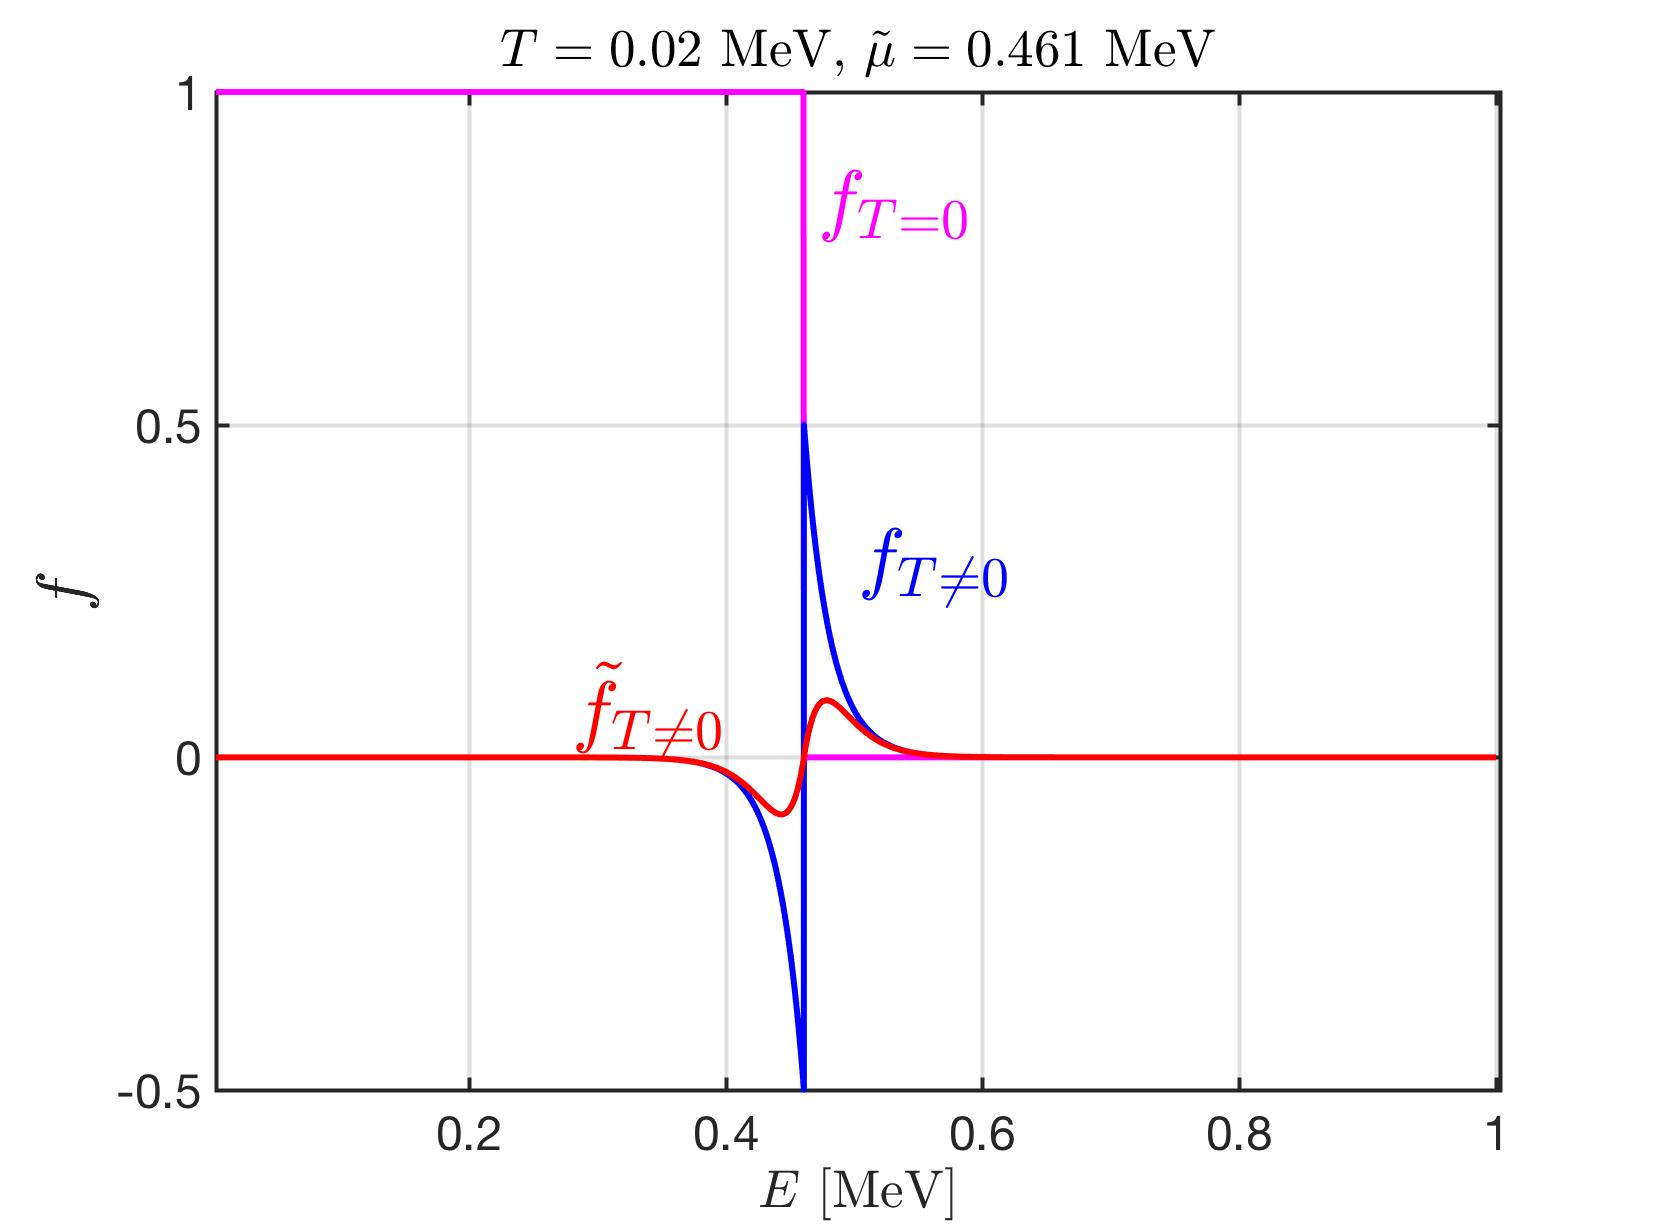
\includegraphics[width=0.5\textwidth]{./plot/FermiZeorFiniteTemperature}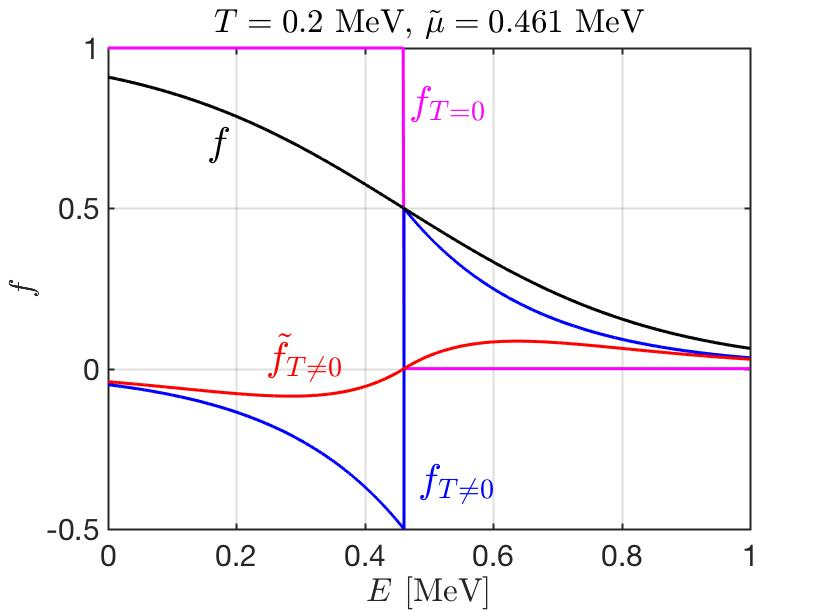
\includegraphics[width=0.5\textwidth]{./plot/FermiZeroFiniteTemperature002}
\caption{%\rev{Here I would add the full fermi distribution - to see how it is decomposed to zero temperature and finite temperature terms.}
The zero and finite temperature components of the decomposition here considered for Fermi distribution as a function of energy with chemical potential $\mu=0.461\MeV$ at temperature $T=0.02\MeV$ and $T=0.2\MeV$. The black line represents the exact Fermi distribution. The purple line represents the zero temperature component $f_{\mathrm{T}=0}$, and blue and red lines represent the finite temperature components $f_\mathrm{T\neq0}$ and $\widetilde f_\mathrm{T\neq0}$ respectively. }
\label{Fermi_Component}
\end{figure}
%%%%%%%%%%%%%%%%%%%%%%%%%%%%%%%%%%%%%%%

The Fig.~\ref{Fermi_Component} shows that the contributions of the two finite temperature components $f_\mathrm{T\neq0}$ and $\widetilde f_\mathrm{T\neq0}$ exponentially decay with the distance from the Fermi surface $E=\mu$. Moreover, the splitting was chosen in such a way that the discontinuous distribution part is fully contained in $f_\mathrm{T\neq 0}$ and $\widetilde{f}_\mathrm{T\neq 0}$ is a remaining continuous function of temperature $T$.  Both finite temperature contributions always have the same sign and lower the distribution for $E < \mu$ and increase it for $E > \mu$.

In contrast to the brute force approach for eliminating the $T=0$ limit from the low-temperature Fermi distribution, our analytic form of distribution offers a more numerically advantageous method for separating the finite temperature components. This is advantage arise from the behavior of: 1.) both finite temperature contributions $f_\mathrm{T\neq0}$ and $\widetilde f_\mathrm{T\neq0}$ always have the same sign 2.) the exponential factor for finite temperature components provide the naturally exponentially suppresses for the large energy. In this scenario, it reduces the numerical noise when evaluate the numerical integral beyond the zero temperature approximation. Furthermore, our novel form for Fermi distribution also provide us the tool to analytically investigate the finite temperature contributions by expanding the function around the Fermi-energy surface, which is useful for addressing physics for the finite temperature approximation.


\section{Asymptotic Expansion of Thermal Averages }
%{\bf As is, this section should probably be removed.  The above calculation suggests that numerical integration will always be an issue, both using  the brute force method and even when using the decomposition, due to the cancellation of leading order terms in $T$ from the integrals of the positive and negative parts.  I think we should replace it with a figure comparing the asymptotic expansion with the numerical integration (which should exhibit instability).  }

To illustrate the advantage of our novel form of distribution can be used to address the integrals common in statistical physics especially when temperature $T\to0$, we examine the thermal average of any given function $G(p)$ . This thermal average physical quantity, denoted as $\langle G\rangle_T$, is determined by integrating over the D-dimensional phase space 
\begin{align}
\langle G\rangle_T&\equiv\int^{\infty}_{0}\!\!\frac{d^Dp}{(2\pi)^D}\,G(p)\,f_{FD}(p)=\frac{1}{(2\pi)^D}\frac{2\pi^{D/2}}{\Gamma(D/2)}\int^{\infty}_{0}\!\!dp\,p^{D-1}\,G(p)\,f_{FD}(p).
\end{align}
By substituting our novel form of FD distribution, the physical quantity $\langle G\rangle_T$ can be expressed as the sum of two distinct components:
\begin{align}
\langle G\rangle_T=\langle G\rangle_{\Theta}+\langle G\rangle_{\Delta T}
\end{align}
 where the $\langle G\rangle_{\Theta}$ corresponds to the zero temperature limit and $\langle G\rangle_{\Delta T}$ represents the finite temperature contribution. We have
\begin{align}
&\langle G\rangle_{\Theta}=\frac{1}{(2\pi)^D}\frac{2\pi^{D/2}}{\Gamma(D/2)}\int^{\infty}_{0}\!\!dp\,p^{D-1}G(p)\Theta\left(\frac{-E+\mu}{T}\right),\qquad E=\sqrt{p^2+m^2},\\
\label{G_deltaT}
&\langle G\rangle_{\Delta T}=\frac{1}{(2\pi)^D}\frac{2\pi^{D/2}}{\Gamma(D/2)}\int^{\infty}_{0}\!\!dp\,p^{D-1}\,G(p)\,\left(f_\mathrm{T\neq0}(p)+\widetilde f_\mathrm{T\neq0}(p)\right).
\end{align}

By employing our decomposition form, we will demonstrate that the integral for finite temperature contribution $\langle G\rangle_{\Delta T}$ can be studied by asymptotic expansion in different regime of interest in physics in following sections. Our novel Fermi distribution can provide the tool to study any physical quantity when temperature approach to zero, and facilitate the connection between the study of finite temperature system to zero temperature limit smoothly. 

%%%%%%%%%%%%%%%%%%%%%%%%%%%%%%%%%%%%%%%%%%%%%%%%%%%%%%%%%%%%%%%%%%%%%%%%%
%\subsection{Asymptotic Expansion of Thermal Averages as $T\to 0$ with $\mu>m$}\label{Appendix:Sommerfeld}
\subsection{Derivation of Sommerfeld expansion: $T\ll m$ with $\mu-m$ not small}\label{Section:Sommerfeld}
{\bf JB: Now that we have the proof that Sommerfeld holds in an appropriate high temp regime, I don't think we need this section anymore.  I think the derivation in the appendix makes the case for the utility of the decomposition and so I don't think we need to redo the usual Sommerfeld derivation, I think it is sufficient to just recall it here.}
In this section we use the decomposition \eqref{Eq_form} naturally leads to an alternative derivation of the Sommerfeld expansion, see, e.g., Eq. (58.1) on page 170 of \cite{landau2013statistical}), i.e., an  asymptotic expansion for the difference between a $D$-dimensional thermal average at finite and zero temperature as $T\to 0$ in the regime where  $\mu>m$.     

{\bf ??To Do: This case can be rephrased in terms of a smooth $H(E)$ and we can simply comment that if one starts with $G(p)$ then the resulting $H(E)$ is smooth because we are assuming $\mu>m$ are fixed. This will make the derivation simpler and should better showcase how the decomposition leads to the Sommerfeld expansion???}
We will assume that $G(p)$, $p\in(0,\infty)$, is a $C^k$ function and that the zeroth through $k$'th derivatives are polynomially bounded.
Start by changing variables to $E=\sqrt{p^2+m^2}$:
\begin{align}
    &\int_0^\infty dp\, p^{D-1} G(p)(f_{T\neq 0}+\widetilde{f}_{T\neq 0})\\
=&\int_0^\infty dp\, p^{D-1} G(p)\frac{1}{2}e^{-|E-\mu|/T}\left\{\mathrm{sgn}(E-\mu)+\tanh[(E-\mu)/(2T)]\right\}\notag\\
    =&\int_m^\infty dE \,Ep^{D-2} G\left(\sqrt{E^2-m^2}\right)\frac{1}{2}e^{-|E-\mu|/T}\left\{\mathrm{sgn}(E-\mu)+\tanh[(E-\mu)/(2T)]\right\}\notag\\
    =&\int_m^{\mu} dE \,E(E^2-m^2)^{(D-2)/2} G\left(\sqrt{E^2-m^2}\right)\frac{1}{2}e^{(E-\mu)/T}\left\{-1+\tanh[(E-\mu)/(2T)]\right\}\notag\\
    &+\int_{\mu}^\infty dE\, E(E^2-m^2)^{(D-2)/2} G\left(\sqrt{E^2-m^2}\right)\frac{1}{2}e^{-(E-\mu)/T}\left\{1+\tanh[(E-\mu)/(2T)]\right\}\,.\notag
\end{align}
Now change variables to $u=(\mu-E)/p_\mu$ in the first integral and $z=(E-\mu)/p_\mu$ in the second where $p_{\mu} \equiv \sqrt{\mu^2 - m^2}$ is the magnitude of the momentum at energy equal to chemical potential. This simplifies the integrands 
\begin{align}
    &\int_0^\infty dp\, p^{D-1} G(p)(f_{T\neq 0}+\widetilde{f}_{T\neq 0})\\
        &=p_\mu^D \int_0^\infty dz\, (z+\widetilde{\mu})[(z+\widetilde{\mu})^2-\widetilde{m}^2]^{(D-2)/2} G\left(p_\mu \sqrt{(z+\widetilde{\mu})^2-\widetilde{m}^2}\right)\frac{1}{1+e^{z/\widetilde{T}}}\notag\\
        &-p_\mu^D \int_0^{\widetilde{\mu}-\widetilde{m}} du\, (\widetilde{\mu}-u)[(\widetilde{\mu}-u)^2-\widetilde{m}^2]^{(D-2)/2} G\left(p_\mu \sqrt{(\widetilde{\mu}-u)^2-\widetilde{m}^2}\right)\frac{1}{1+e^{u/\widetilde{T}}}\,,\notag
\end{align}
where 
\begin{equation}
\widetilde{T} \equiv T/p_\mu, \quad \widetilde{\mu} \equiv \mu/p_\mu, \quad  \widetilde{m} \equiv m/p_\mu     
\end{equation}
are dimensionless quantities. Define
\begin{align}\label{eq:F_tilde_F_def}
  &F(z,\wt{m},\wt{\mu}) \equiv (z+\wt{\mu})[(z+\wt{\mu})^2-\wt{m}^2]^{(D-2)/2} G\left(p_\mu\sqrt{(z+\wt{\mu})^2-\wt{m}^2}\right)\,,\,\,\,z\in[0,\infty)\,,\\ 
  &\hat{F}(u,\wt{m},\wt{\mu}) \equiv (\wt{\mu}-u)[(\wt{\mu}-u)^2-\wt{m}^2]^{(D-2)/2} G\left(p_\mu\sqrt{(\wt{\mu}-u)^2-\wt{m}^2}\right)\,,\,\,\, u\in[0,\wt{\mu}-\wt{m}]\,.\notag
\end{align}
The assumptions on $G$ allow us to obtain   Taylor expansions with remainder in $z$ and $u$ respectively:
\begin{align}\label{eq:a_a_tilde_def}
F(z,\wt{m},\wt{\mu})=&\sum_{n=0}^{k-1} a_{n}(\wt{m},\wt{\mu})z^n + R_k(z,\wt{m},\wt{\mu})\,,\,\,\, a_n(\wt{m},\wt{\mu})\equiv\frac{1}{n!}\partial_z^nF(0,\wt{m},\wt{\mu})\,,\\
\hat{F}(u,\wt{m},\wt{\mu})=&\sum_{n=0}^{k-1} \hat{a}_{n}(\wt{m},\wt{\mu})u^n + \hat{R}_k(u,\wt{m},\wt{\mu})\,,\,\,\,\hat{a}_n(\wt{m},\wt{\mu})\equiv\frac{1}{n!}\partial_u^n\hat{F}(0,\wt{m},\wt{\mu})\,,\notag
\end{align}
where the remainders satisfy polynomial growth bounds of the form 
\begin{align}\label{eq:remainder_bounds}
&|R_k(z,\wt{m},\wt{\mu})|\leq z^k(\alpha_k(\wt{m},\wt{\mu})+\beta_k(\wt{m},\wt{\mu}) z^{q_k})\,,\\
&|\hat{R}_k(u,\wt{m},\wt{\mu})|\leq u^k(\hat{\alpha}_k(\wt{m},\wt{\mu})+\hat{\beta}_k(\wt{m},\wt{\mu}) u^{\hat{q}_k})\notag
\end{align}
for some coefficients $\alpha_k,\beta_k,\hat{\alpha}_k,\hat{\beta}_k$ and powers $q_k$, $\hat{q}_k$.
 Note that the assumption $\mu>m$ ensures that the square roots and powers do not introduce any singularities at $0$ in the formulas for $F$ and $\widetilde F$ and therefore the required derivatives of $F$ and $\hat{F}$ exist when $G(p)$ is sufficiently smooth.   The definitions \eqref{eq:F_tilde_F_def} are in fact both valid on a neighborhood on $0$ and there one has the relationship $\hat{F}(u,\wt{m},\wt{\mu})=F(-u,\wt{m},\wt{\mu})$. Therefore one finds  $\hat{a}_n=(-1)^n{a}_n$ for all $n$. The remainder terms in \req{eq:a_a_tilde_def} are given by
 \begin{align}
    R_k(z,\wt{m},\wt{\mu})=& z^k\int_0^1\frac{(1-s)^{k-1}}{(k-1)!}\partial^k_{z}F(sz,\wt{m},\wt{\mu})ds\,,\\
       \hat{R}_k(u,\wt{m},\wt{\mu})=& u^k\int_0^1\frac{(1-s)^{k-1}}{(k-1)!}\partial^k_{u}\hat{F}(su,\wt{m},\wt{\mu})ds\notag
 \end{align}
and so the bounds \eqref{eq:remainder_bounds} follow from polynomially boundedness of   $\partial_z^k F$ and $\partial_u^k \hat{F}$,  which in turn follows from polynomial boundedness of the zeroth through $k$'th derivatives of $G$.  We note that if one is only interested in the asymptotic behavior, and not in an explicit error bound, then the $\alpha_k,\beta_k,\hat{\alpha}_k,\hat{\beta}_k$ and powers $q_k$, $\hat{q}_k$ do not need to be computed.  
 
Recalling the integral formulas
\begin{align}\label{eq:FD_power_integrals}
    \int_0^\infty \frac{x^{\nu-1}}{e^{ x}+1}dx=\begin{cases}
    \ln(2) &\,, \,\,\text{ if }\nu=1\\
        (1-2^{1-\nu})\Gamma(\nu)\zeta(\nu)  &\,, \,\,\nu\in(1,\infty)
    \end{cases}
\end{align}
(see 3.411.3 on page 353 of  \cite{Gradshteyn:1943cpj}). Using \eqref{eq:FD_power_integrals} we compute the following:
\begin{align}
 &\int_0^\infty dz\, F(z,\wt{m},\wt{\mu})\frac{1}{1+e^{z/\wt{T}}}\\
 =& \sum_{n=0}^{k-1} a_{n}(\wt{m},\wt{\mu})\int_0^\infty dz\, z^n \frac{1}{1+e^{z/\wt{T}}}+ \int_0^\infty dz\, R_k(z,\wt{m},\wt{\mu})\frac{1}{1+e^{z/\wt{T}}}\notag\\
 =&\ln(2)a_0(\widetilde{m},\widetilde{\mu})\widetilde{T} +\sum_{n=1}^{k-1} a_{n}(\wt{m},\wt{\mu})\wt{T}^{n+1}(1-2^{-n})\Gamma(n+1)\zeta(n+1)\notag\\
 &+ \int_0^\infty dz\, R_k(z,\wt{m},\wt{\mu})\frac{1}{1+e^{z/\wt{T}}}\,,\notag
\end{align}
where the integral of the remainder has the bound
\begin{align}
  &\left|\int_0^\infty dz\, R_k(z,\wt{m},\wt{\mu})\frac{1}{1+e^{z/\wt{T}}}\right|\\
  \leq &   \int_0^\infty dz\,z^k[\alpha_k(\wt{m},\wt{\mu})+\beta_k(\wt{m},\wt{\mu}) z^{q_k}]\frac{1}{1+e^{z/\wt{T}}}\notag\\
  =& \alpha_k(\wt{m},\wt{\mu}) \wt{T}^{k+1}(1-2^{-k})\Gamma(k+1)\zeta(k+1)\notag\\
  &+\beta_k(\wt{m},\wt{\mu}) \wt{T}^{k+q_k+1}(1-2^{-(k+q_k)})\Gamma(k+q_k+1)\zeta(k+q_k+1)\notag\\ 
  =&\mathcal{O}(\wt{T}^{k+1})\,.\notag
\end{align}
Similarly we have
\begin{align}
    &\int_0^{\wt{\mu}-\wt{m}} du\,\hat{F}(u,\wt{m},\wt{\mu})\frac{1}{1+e^{u/\wt{T}}}\\
    =&\sum_{n=0}^{k-1} \hat{a}_{n}(\wt{m},\wt{\mu})\int_0^{\wt{\mu}-\wt{m}} du \,u^n  \frac{1}{1+e^{u/\wt{T}}}+ \int_0^{\wt{\mu}-\wt{m}} du\,\hat{R}_k(u,\wt{m},\wt{\mu}) \frac{1}{1+e^{u/\wt{T}}}    \notag\\
        =&\sum_{n=0}^{k-1} \hat{a}_{n}(\wt{m},\wt{\mu})
        T^{n+1}(1-2^{-n})\Gamma(n+1)\zeta(n+1)      
        + \int_0^{\wt{\mu}-\wt{m}} du\,\hat{R}_k(u,\wt{m},\wt{\mu}) \frac{1}{1+e^{u/\wt{T}}}    \notag\\
        &-\sum_{n=0}^{k-1} \hat{a}_{n}(\wt{m},\wt{\mu})\int_{\wt{\mu}-\wt{m}}^\infty du\, u^n  \frac{1}{1+e^{u/\wt{T}}}\,,\notag
\end{align}
where
\begin{align}
&\left|\int_0^{\wt{\mu}-\wt{m}} du\, \hat{R}_k(u,\wt{m},\wt{\mu})\frac{1}{1+e^{u/\wt{T}}}\right|\\
\leq &\int_0^\infty u^k[\hat{\alpha}_k(\wt{m},\wt{\mu})+\hat{\beta}_k(\wt{m},\wt{\mu}) u^{\hat{q}_k}]\frac{1}{1+e^{u/\wt{T}}}\notag\\
\leq&\hat{\alpha}_k(\wt{m},\wt{\mu}) \wt{T}^{k+1}(1-2^{-k})\Gamma(k+1)\zeta(k+1)\notag\\
  &+\hat{\beta}_k(\wt{m},\wt{\mu}) \wt{T}^{k+\hat{q}_k+1}(1-2^{-(k+\hat{q}_k)})\Gamma(k+\hat{q}_k+1)\zeta(k+\hat{q}_k+1) \notag\\
  =&\mathcal{O}(\wt{T}^{k+1})\notag
\end{align}
and
\begin{align}\label{eq:exp_supressed_remainder}
\left|\sum_{n=0}^{k-1} \hat{a}_{n}(\wt{m},\wt{\mu})\int_{\mu-m}^\infty du\, u^n  \frac{1}{1+e^{u/\wt{T}}}\right|
\leq&\sum_{n=0}^{k-1} |\hat{a}_{n}(\wt{m},\wt{\mu})|\int_{\mu-m}^\infty du\, u^n  e^{-u/\wt{T}}\\
=&\sum_{n=0}^{k-1} |\hat{a}_{n}(\wt{m},\wt{\mu})|T^{n+1}\Gamma(n+1,(\wt{\mu}-\wt{m})/\wt{T})\,.\notag
\end{align}
Here $\Gamma(s,x)$ is the incomplete Gamma function which has the asymptotic behavior $\Gamma(s,x)=\mathcal{O}(e^{-x}x^{s-1})$ as $x\to\infty$ and hence \eqref{eq:exp_supressed_remainder} decays exponentially as $\wt{T}\to 0$, as compared to the other remainder terms which decay polynomially in $\wt{T}$.  

Putting the above calculations together, when $m<\mu$ and $G(p)$ is smooth with polynomially bounded zeroth through $k$'th derivatives we obtain the following asymptotic result as $T\to 0$:
\begin{align}
    &\int_0^\infty dp\, p^{D-1} G(p)(f_{T\neq 0}+\widetilde{f}_{T\neq 0})\\
    =& 2p_\mu^D\sum_{n=1, \text{odd}}^{k-1} 
        (1-2^{-n})\Gamma(n+1)\zeta(n+1){a}_n(\wt{m},\wt{\mu})\wt{T}^{n+1}+ \mathcal{O}(\wt{T}^{k+1})\,,\notag\\
        &a_n(\wt{m},\wt{\mu})=\frac{1}{n!}\partial_z^n|_{z=0} \left[(z+\wt{\mu})[(z+\wt{\mu})^2-\wt{m}^2]^{(D-2)/2} G\left(p_\mu\sqrt{(z+\wt{\mu})^2-\wt{m}^2}\right)\right]\,.\notag
\end{align}
Here we used the fact that   $\hat{a}_n=(-1)^n{a}_n$ for all $n$ to cancel the even terms in the sum. Note that the implied constant in the error bound depends on $m$ and $\mu$, and also on any parameters that enter into $G$; the error term can be explicitly bounded using the  formulas derived above.

Specifically, for $D=3$ the expansion in temperature starts as
\begin{equation}\label{eq:Sommerfeld_expansion}
    \begin{split}
    \int_0^\infty &dp\, p^2 G(p) (f_{T\neq 0} + \widetilde{f}_{T\neq 0})\\
    &= \frac{\pi^2}{6} p_\mu^3\left[(1 + \wt{\mu}^2)G(p_{\mu}) + \wt{\mu}^2  \wt{G}'(p_{\mu})\right] \wt{T}^2 \\
    &+ \frac{7\pi^4}{360}p_\mu^3\left[3\wt{m}^4 G(p_{\mu}) + 3(2-\wt{m}^4)\wt{G}'(p_{\mu})+ 6\wt{\mu}^2 \wt{G}''(p_{\mu}) + \wt{\mu}^4 \wt{G}'''(p_{\mu})\right]\wt{T}^4\\
    &+ \mathcal{O}(\wt{T}^6)\,,
    \end{split}
\end{equation}
where the re-scaled unitless derivatives denoted by prime are 
\begin{equation}
    \wt{G}^{(n)}(p_\mu) \equiv p_\mu^n \left.\frac{\partial^{n}}{\partial p^{n}} G(p)\right|_{p = p_\mu}
\end{equation}
Note that integrals over energy can be converted to this type of integral by change of variables $p dp = E dE$
\begin{equation}
    \int_m^\infty dE f_{FD}(E) H(E) = \int_0^\infty p^2 dp \frac{H(p)}{p\sqrt{p^2 + m^2}}f_{FD}(p) 
\end{equation}
where $G(p) = H(p)/(p\sqrt{p^2+m^2})$. Substituting to the first order term in \req{eq:expansion} the terms which do not contain derivative of $H(p)$ exactly cancel and we obtain
\begin{equation}
    \int_m^\infty dE (f_{T\neq 0}+\widetilde{f}_{T\neq 0})(E)H(E) = \frac{\pi^2}{6} \left.\frac{dH(E)}{dE}\right|_{E=\mu} T^2 + \mathcal{O}(T^4)
\end{equation}
which is the Sommerfeld low-temperature expansion \cite{landau2013statistical}. For this derivation note that
\begin{equation}
    \left. \frac{dH(p)}{dp}\right|_{p=p_\mu} = \left.\frac{1}{\wt{\mu}}\frac{dH(E)}{dE}\right|_{E=\mu}
\end{equation}



%%%%%%%%%%%%%%%%%%%%%%%%%%%%%%%%%%%%%%%%%%%%%%%%%%%%%%%%%%%%%%%%%%%%%%%%%
\subsubsection{Numerical illustration: $G(p)=1$}
To illustrate the benefits of our innovative Fermi distribution function in practical applications, we examine the partition function for semi-relativistic electron with a chemical potential $\mu>m$ as an example. We consider the integral in $3$-dimension phase space with weight function $G(p)=1$. The exact with exact Fermi-Dirac distribution is give by
\begin{align}\label{lnZ_Exact}
I_{\mathrm{FD}}\equiv\int\frac{d^3p}{(2\pi)^3}\frac{1}{e^{(E-\mu)/T}+1}.
\end{align}

On the other hand, using the novel form of Fermi-Dirac distribution and asymptotic expansion, the  integral can be written as
\begin{align}\label{lnZ_Sum}
I_{\mathrm{Asym}}=\left[I_{\Theta}+I_{\wt{T}^2}+I_{\wt{T}^4}+\mathcal{O}(\wt{T}^6)\right]
\end{align}
where the functions $I_\Theta$, $I_{\wr{T}^2}$, and $I_{\wt{T}^4}$ are given by
\begin{align}
&I_\Theta=\frac{1}{2\pi^2}\int^{\infty}_{0}\!\!dp\Theta\left(\frac{-E+\mu}{T}\right),\\
&I_{\wt{T}^2}=\frac{p_\mu^3}{12\pi^2}(1 + \wt{\mu}^2)G(p_{\mu})\wt{T}^2,\\
&I_{\wt{T}^4}=\frac{7\pi^2}{120}p_\mu^3\wt{m}^4 G(p_{\mu})\wt{T}^4.
\end{align}

To demonstrate the equivalence between our novel distribution and the Fermi-Dirac distribution for the partition function, we take the ratio between Eq.~(\ref{lnZ_Sum}) and Eq.~(\ref{lnZ_Exact}) we have
\begin{align}\label{lnZ_Ratio}
\frac{I_\mathrm{Asym}}{I_\mathrm{FD}}=\frac{I_{\Theta}+I_{\wt{T}^2}+I_{\wt{T}^4}+\mathcal{O}(\wt{T}^6)}{I_\mathrm{FD}}
\end{align}
%%%%%%%%%%%%%%%%%%%%%%%%%%%%%%%%%%%%%%%
\begin{figure}[t]
\centering
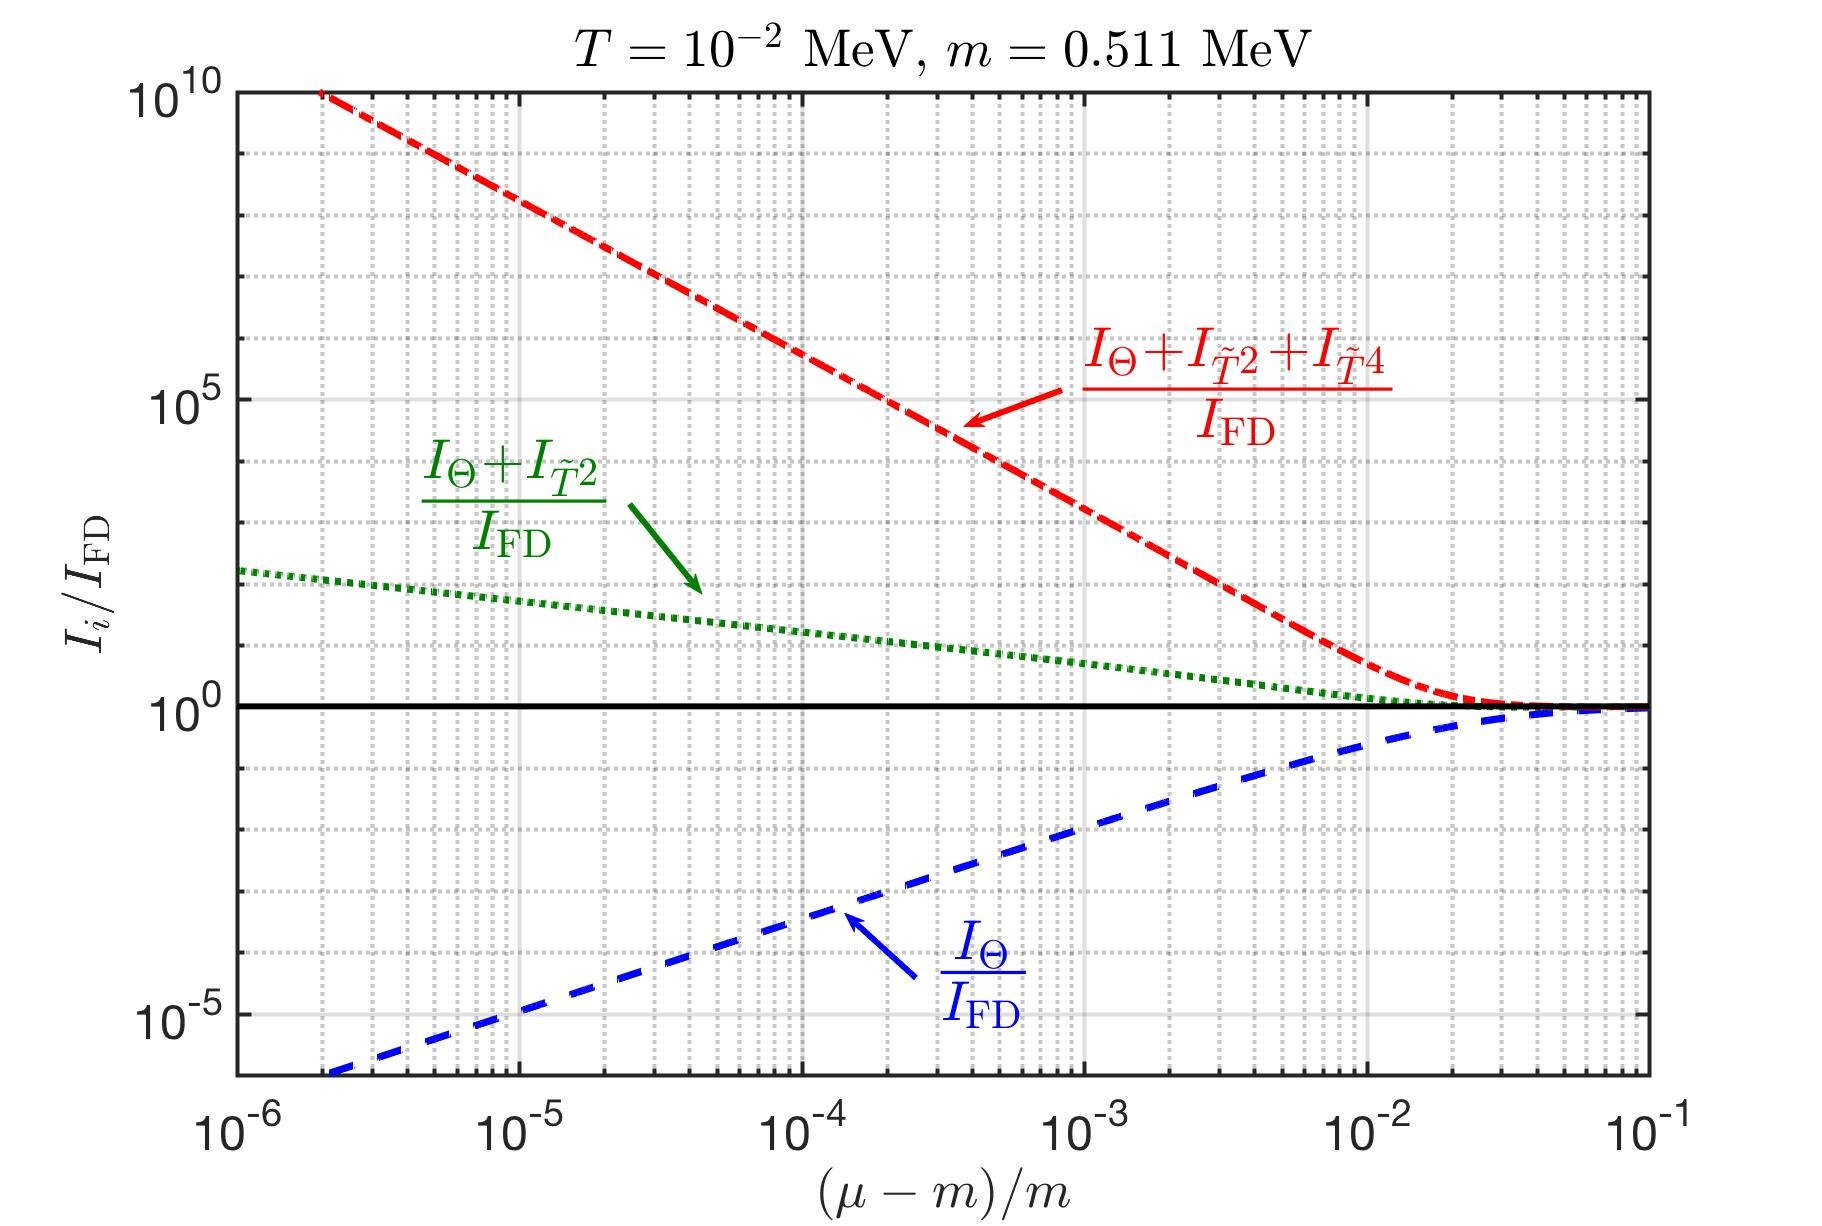
\includegraphics[width=0.5\textwidth]{./plot/Lowmu_T2}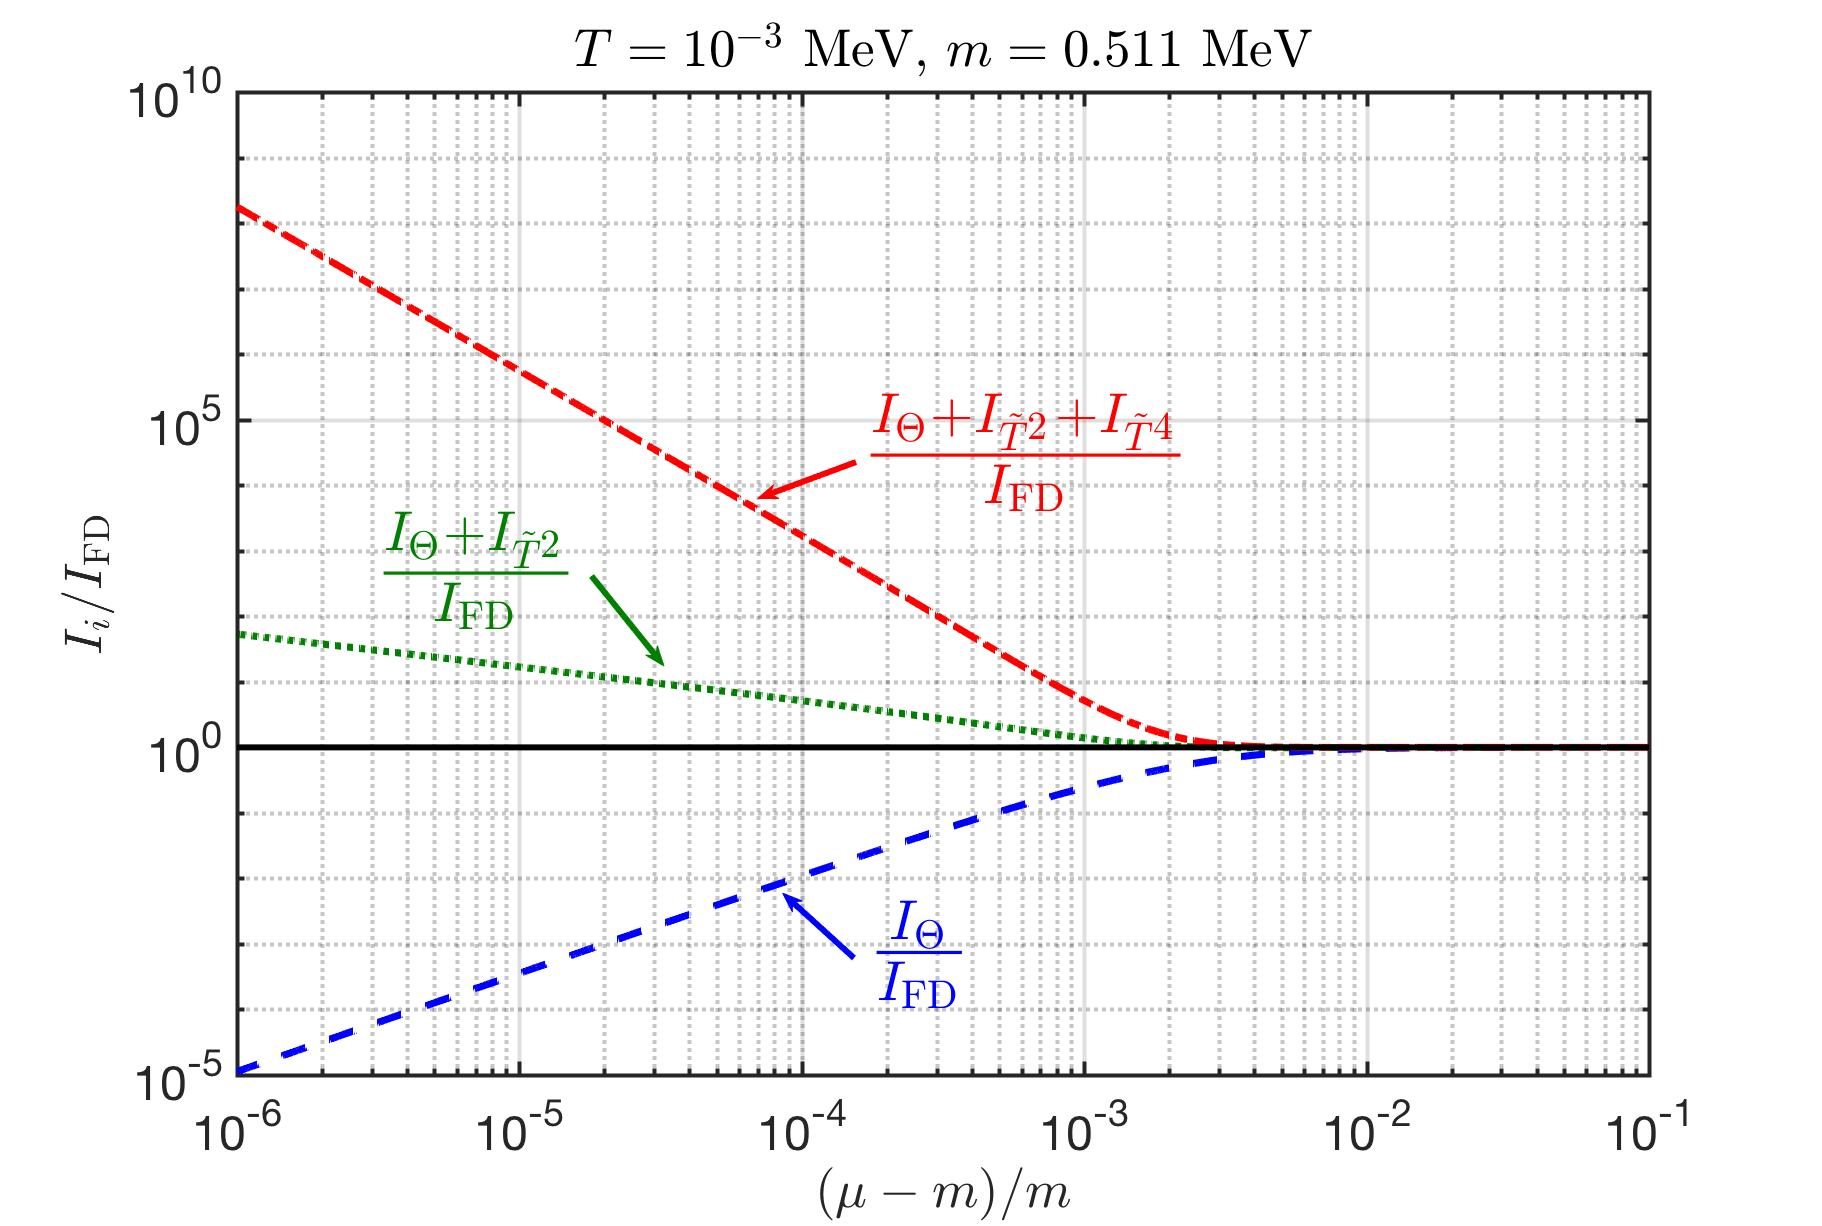
\includegraphics[width=0.5\textwidth]{./plot/Lowmu_T3}\\
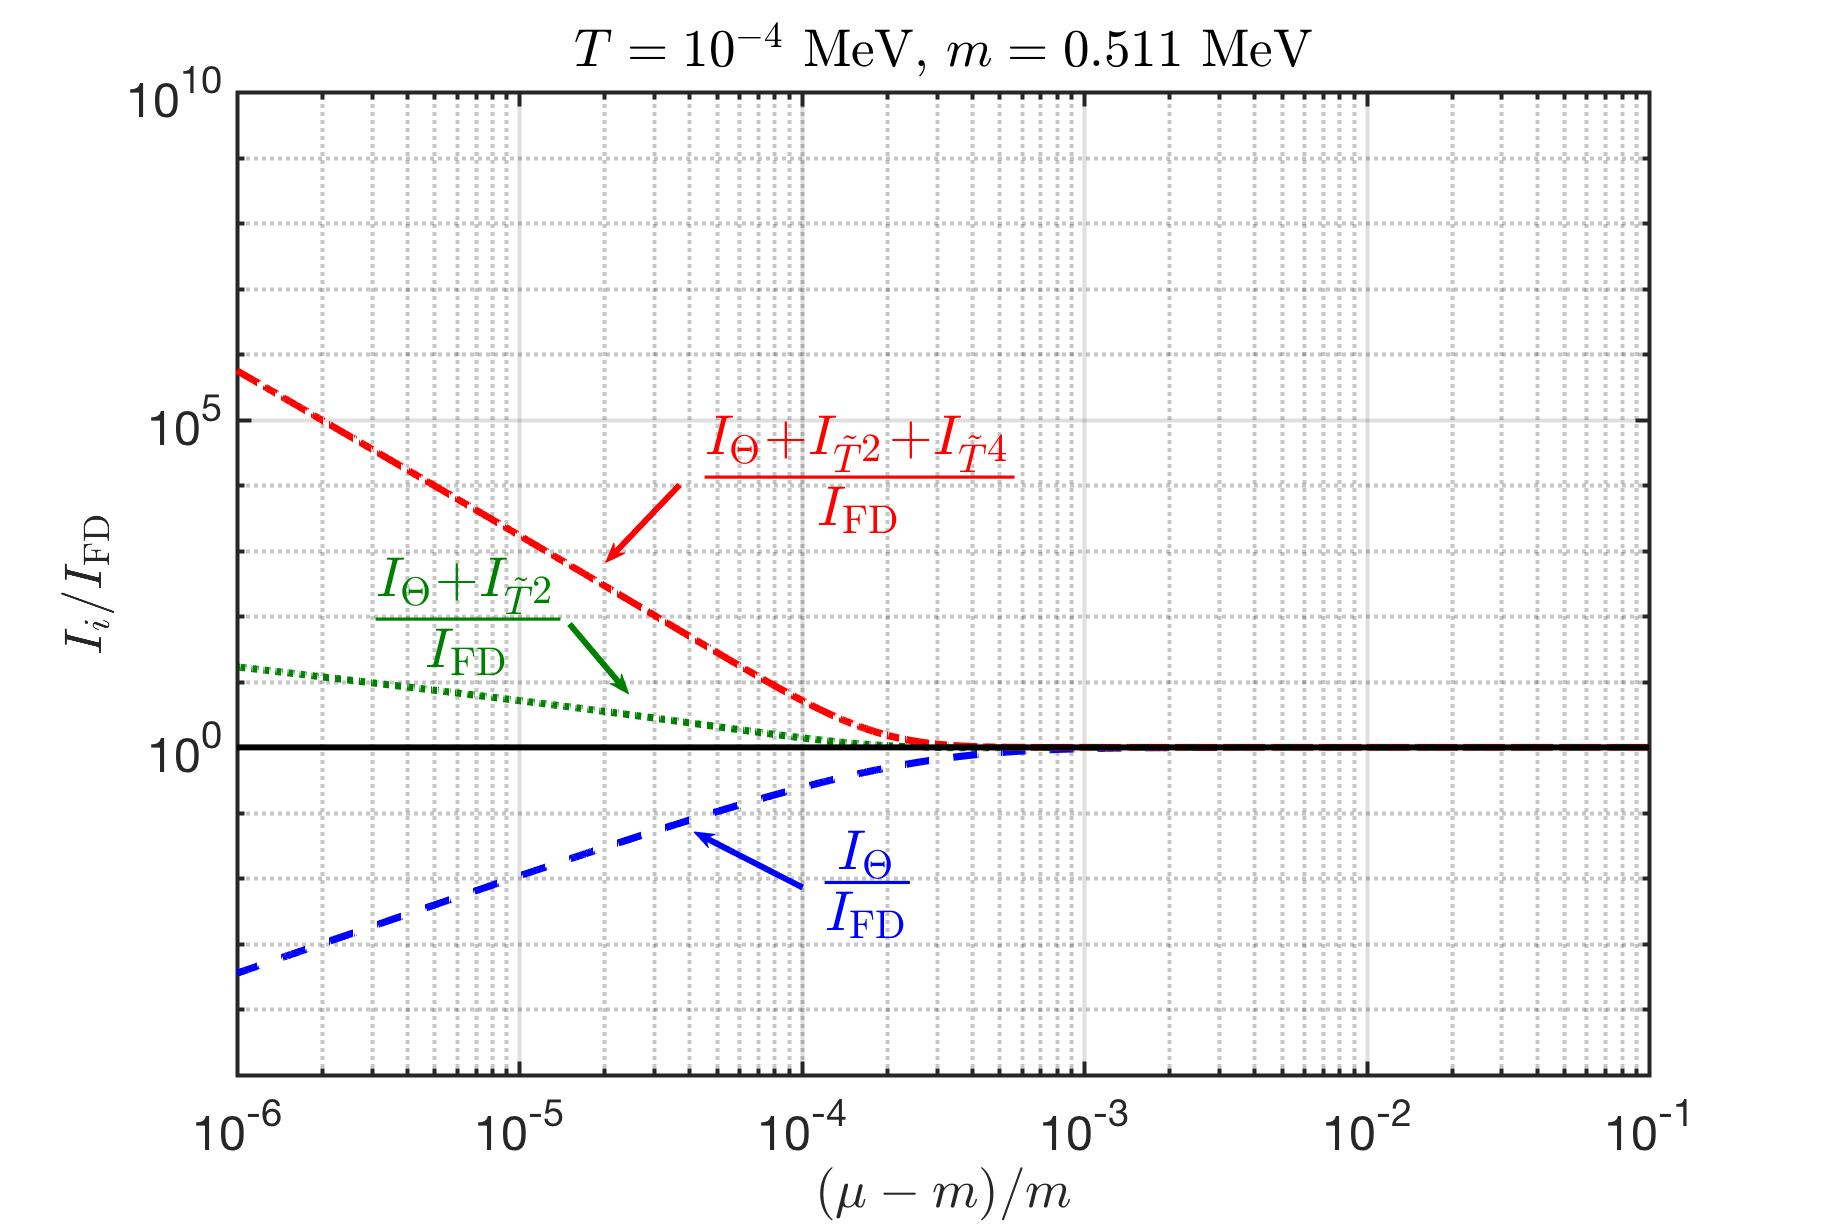
\includegraphics[width=0.5\textwidth]{./plot/Lowmu_T4}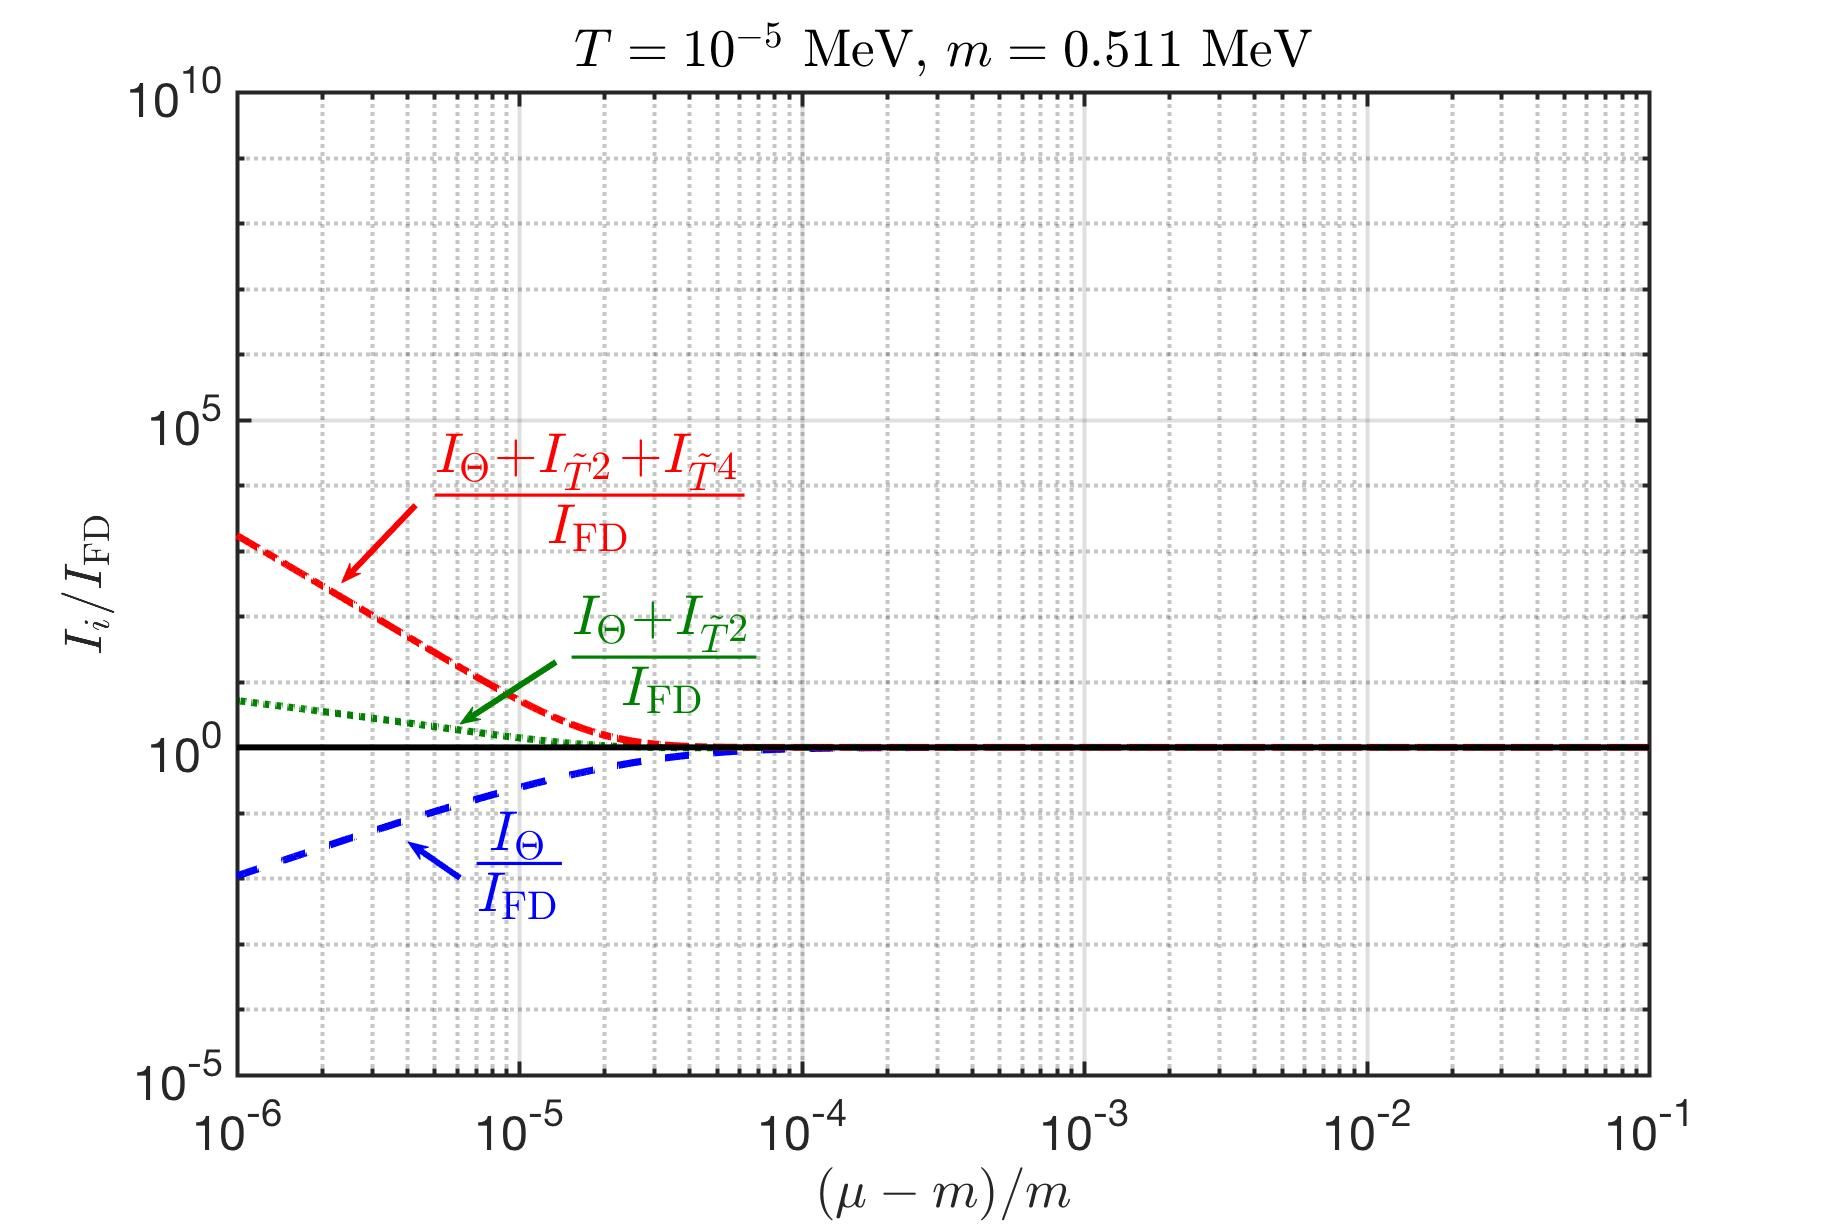
\includegraphics[width=0.5\textwidth]{./plot/Lowmu_T5}
\caption{ The ratio between numerical integral Eq.~(\ref{lnZ_Ratio}) as a function of chemical potential $(\mu-m)/m$ with different temperature  {\bf Somewhere we should point out that adding more terms doesn't necessarily help because it is an asymptotic expansion, not convergent.  I think the best comparison for us to make with with the expansion \eqref{thm:mu_zero_faster} and to reverse the roles of $T$ and $\mu$ (i.e., $x$-axis of plots shows $(\mu-m)/m$ with several plots for several different $T$'s. The example $G(p)=1$ should suffice: see figures \ref{fig:Thm3_vs_Sommerfeld_comparison_fixed_T} (\ref{fig:FD_avg_expansion_comparison_Sommerfeld}is another way of displaying the comparison) }}
\label{lnZ_Ratio_fig}
\end{figure}
\begin{figure}
\centering
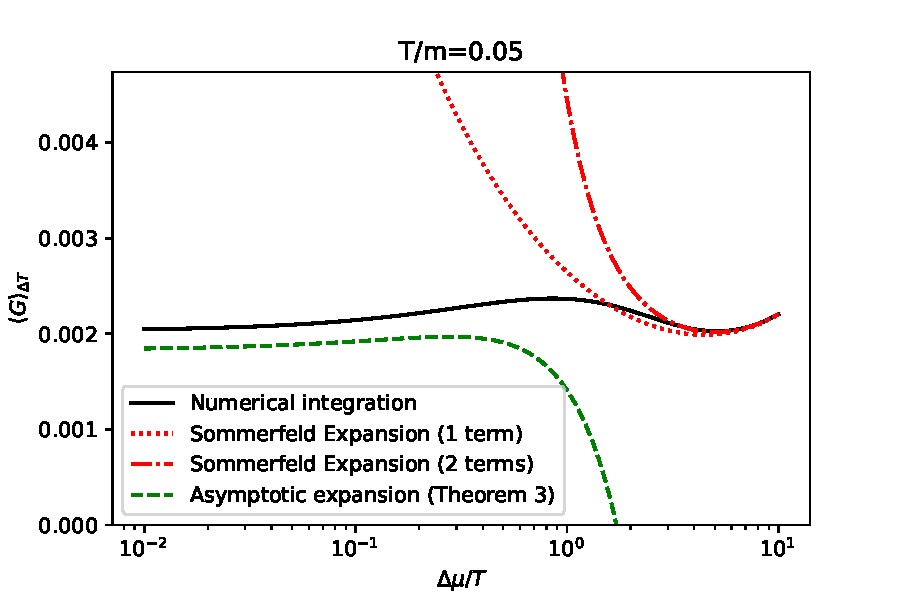
\includegraphics[width=0.49\textwidth]{./plot/Thm3_vs_Sommerfeld_comparison_T_0.05m.pdf}
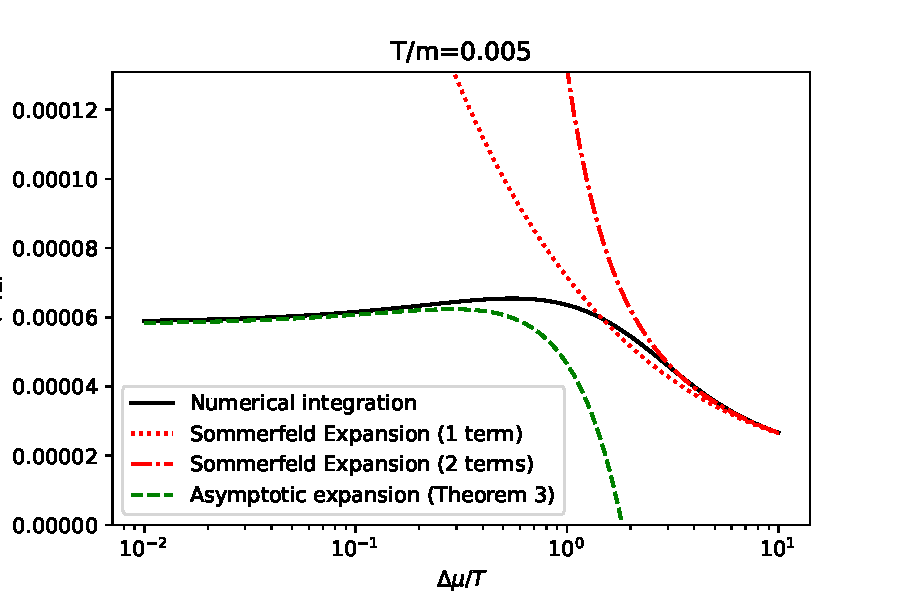
\includegraphics[width=0.49\textwidth]{./plot/Thm3_vs_Sommerfeld_comparison_T_0.005m.pdf}
\caption{Comparison of $\langle G\rangle_{\Delta T}$ for $G(p)=1$, as approximated by the classical Sommerfeld formula (red curves) and our Theorem \ref{thm:mu_zero_faster} (green curves).  The theory states that Sommerfeld applies when $T\to 0$ and $\Delta\mu$ is not small, while Theorem \ref{thm:mu_zero_faster} applies when $\Delta\mu\ll T\ll m$. We see these regimes reflected in the figure, with Sommerfeld more accurate as $\Delta\mu/T$ increases above $1$ and the result of Theorem \ref{thm:mu_zero_faster} more accurate as $\Delta\mu/T$ decreases below $1$.}\label{fig:Thm3_vs_Sommerfeld_comparison_fixed_T}
\end{figure}

%%%%%%%%%%%%%%%%%%%%%%%%%%%%%%%%%%%%%%%
In Fig.~\ref{lnZ_Ratio_fig} we plot the ratio between numerical integral Eq.~(\ref{lnZ_Ratio}) as a function of chemical potential $(\mu-m)/m$ with different temperature. It shows that the Sommerfeld expansion is asymptotic in nature \cite{landau2013statistical}, meaning that adding further terms does not necessarily reduce the error at fixed values of $T$ and $\mu$.  This is particularly relevant when $\mu-m$ is small, a regime that the classical Sommerfeld expansion was not designed for. When dealing with multiple scales, here $T$ and $\mu-m$, one generally requires specialized asymptotic expansions that are adapted to regime under consideration. Furthermore, expanding the Sommerfeld result around the small chemical potential may lead to encountering singularities which underscore the necessity for a better tool to study this scenario. In following section, we will demonstrate that our novel Fermi distribution function serves as a valuable tool for studying Fermi gases with small chemical potentials in the low temperature regime.







%%%%%%%%%%%%%%%%%%%%%%%%%%%%%%%%%%%%%%%


% Martin - Highlight the method can be used to address the integrals common in stastistical physics.
% Johann - First time we separate cleanly the hot and cold components. This therefore could be very useful for studying interacting systems where the mathematics becomes intractible quickly. The properties near to the Fermi surface are clearly isolated and most of the interactions occur near the Fermi surface.
% Cold matter cannot form pairs, but finite temperature systems can because of the deformation of the step function. Particle-antiparticle hope pairs behavior is isolated. May have applications to superconducting systems. Allowing for the exploration of interacting systems at the Fermi surface.
% Reference to superconducting neutron stars.
% Andrew - This allows us to analyze the finite temperature elements as a distinct model.
% Cheng Tao - This novel form is numerically friendly as the finite temperature components are naturally exponentially suppresses while also preserving the sign of all corrections making the formulation easier to numerically integrate.

%%%%%%%%%%%%%%%%%%%%%%%%%%%%%%%%%%%%%%%

%\subsection{Asymptotic Expansion of Thermal Averages in the regime $T=\mathcal{O}(\mu-m)$}\label{sec:asymp_T_0_faster}
\subsection{Asymptotic Expansion in the regime: $T=\mathcal{O}(\mu-m)$}\label{sec:asymp_T_0_faster}

In this section we use the decomposition \eqref{Eq_form} to obtain an asymptotic expansion for the difference between a $D$-dimensional thermal average ($D\geq 2$) at finite and zero temperature when $T$ approaches zero at a faster rate than $\mu$ approaches $m$.   More specifically, we will assume 
\begin{align}\label{eq:T_mu_relation}
    \mu=m+\Delta\mu\,, \,\Delta\mu>0 \,\, \text{ and } \,\, \widetilde{T}=d\Delta\widetilde{\mu}^{1+\gamma}\,, \,\,d,\gamma>0\,,
\end{align}
where $\widetilde{T}\equiv T/m$ and $\Delta\widetilde{\mu}\equiv \Delta\mu/m$. We will study the limit $\Delta\widetilde{\mu}\to 0^+$.



 Let $G(p)$, $p\in[0,\infty)$, be a $C^k$ function whose zeroth through $k$'th derivatives are polynomially bounded and begin by changing variables to $E=\sqrt{p^2+m^2}$:
\begin{align}
    &\int_0^\infty dp\, p^{D-1} G(p)(f_{T\neq 0}+\widetilde{f}_{T\neq 0})\notag\\
=&\int_0^\infty dp\, p^{D-1} G(p)\frac{1}{2}e^{-|E-\mu|/T}\left\{\mathrm{sgn}(E-\mu)+\tanh[(E-\mu)/(2T)]\right\}\notag\\
    =&\int_m^\infty dE \,Ep^{D-2} G\left(\sqrt{E^2-m^2}\right)\frac{1}{2}e^{-|E-\mu|/T}\left\{\mathrm{sgn}(E-\mu)+\tanh[(E-\mu)/(2T)]\right\}\notag\\
    =&\int_{\mu}^\infty dE\, E(E^2-m^2)^{(D-2)/2} G\left(\sqrt{E^2-m^2}\right)
    \frac{1}{1+e^{(E-\mu)/T}}\label{eq:2_int_decomp_T_faster}  \\
    &-\int_m^{\mu} dE \,E(E^2-m^2)^{(D-2)/2} G\left(\sqrt{E^2-m^2}\right)\frac{1}{1+e^{(\mu-E)/T}} \,.\notag
\end{align}
Next consider the first integral in \eqref{eq:2_int_decomp_T_faster}. In general, its integrand will have a singularity at $E=m$. As the lower limit of integration approaches $m$ in the regime under consideration, it is necessary to carefully resolve that singularity. We have chosen to begin with the integral expressed in terms of $p$ because it simplifies this analysis, due to $E=\sqrt{p^2+m^2}$ being is a smooth function of $p$ but not vice versa. Thus if one begins with a smooth density of states $H(E)$, the corresponding $G(p)$ will also be smooth but the reverse is not true. We note that if one is interested in $G(p)$ that is not smooth at $p=0$ then the following derivation would need to be modified to account for this.

To derive an expansion that correct handles the singular behavior of the integrands in \eqref{eq:2_int_decomp_T_faster} at $E=m$, we first change variables to $z=(E-m)/m$  to obtain
\begin{align}
&\int_{\mu}^\infty dE\, E(E^2-m^2)^{(D-2)/2} G\left(\sqrt{E^2-m^2}\right)
    \frac{1}{1+e^{(E-\mu)/T}}\notag   \\
    =&m^{D}\int_{\Delta\widetilde{\mu}}^\infty dz\, (z+1)((z+1)^2-1)^{(D-2)/2} G\left(m\sqrt{(z+1)^2-1}\right)
    \frac{1}{1+e^{(z-\Delta\widetilde{\mu})/\widetilde{T}}} \notag\\
        =&m^{D}\int_{\Delta\widetilde{\mu}}^\infty dz\, \left[(z+1)(  z+2)^{(D-2)/2} G\left(m\sqrt{z}\sqrt{z+2}\right)\right]
    \frac{z^{(D-2)/2}}{1+e^{(z-\Delta\widetilde{\mu})/\widetilde{T}}} \,.\label{eq:T_faster_int_1_change_vars}
\end{align}
We have separated out the (possible) singuarlity coming from $z^{(D-2)/2}$ but there still remains a potential singularity at $z=0$ coming from the argument of  $G$. Therefore the term in brackets does not always have a Taylor expansion, but it does have a more general asymptotic expansion which we can obtain a follows.  Define  
\begin{align}\label{eq:F_y_m_def}
  F(y,m)\equiv  (y^2+1)(  y^2+2)^{(D-2)/2} G\left(my\sqrt{y^2+2}\right)\,.
\end{align}
We have assumed that $G$ is $C^k$ on $[0,\infty)$ with polynomially bounded zeroth through $k$'th derivatives and therefore $y\mapsto F(y,m)$ also has these properties.  We can therefore use Taylor's theorem with remainder to write
\begin{align}\label{eq:F_y_m_Taylor}
F(y,m)=&\sum_{n=0}^{k-1} a_n(m)y^n +R_k(y,m)\,, \,\,\,a_n(m)=\frac{1}{n!}\partial_y^n F(0,m)\,,
\end{align}
where the remainder term is given by
\begin{align}
R_k(y,m)=y^k \int_0^1\frac{(1-s)^{k-1}}{(k-1)!}\partial_y^k F(sy,m)ds
\end{align}
and can be bounded via
\begin{align}\label{eq:R_k_poly_bound}
|R_k(y,m)|\leq y^k[\alpha_k(m)+\beta_k(m)y^{q_k}]
\end{align}
for some coefficients $\alpha_k,\beta_k$ and power $q_k$.

With this we have
\begin{align}
\eqref{eq:T_faster_int_1_change_vars} =&m^{D}\int_{\Delta\widetilde{\mu}}^\infty dz\, F(\sqrt{z},m)    \frac{z^{(D-2)/2}}{1+e^{(z-\Delta\widetilde{\mu})/\widetilde{T}}} \\
=& \sum_{n=0}^{k-1} a_n(m)m^{D}\int_{\Delta\widetilde{\mu}}^\infty dz\, \frac{z^{(n+D-2)/2}}{1+e^{(z-\Delta\widetilde{\mu})/\widetilde{T}}}+m^{D}\int_{\Delta\widetilde{\mu}}^\infty dz\,R_k(\sqrt{z},m)\frac{z^{(D-2)/2}}{1+e^{(z-\Delta\widetilde{\mu})/\widetilde{T}}}\,.\notag
\end{align}
The remainder term can be bounded by using \eqref{eq:R_k_poly_bound} as follows
\begin{align}
   &\left|m^{D}\int_{\Delta\widetilde{\mu}}^\infty dz\,R_k(\sqrt{z},m)\frac{z^{(D-2)/2}}{1+e^{(z-\Delta\widetilde{\mu})/\widetilde{T}}}\right|\\
   \leq&m^{D}\int_{\Delta\widetilde{\mu}}^\infty dz\,z^{k/2}[\alpha_k(m)+\beta_k(m)z^{q_k/2}]z^{(D-2)/2}e^{-(z-\Delta\widetilde{\mu})/\widetilde{T}}\notag\\
=&d\alpha_k(m)m^{D}\Delta\widetilde{\mu}^{(k+D)/2+\gamma}\int_{0}^\infty dx\,(1+d\Delta\widetilde{\mu}^{\gamma}x)^{(k+D-2)/2}e^{-x}\notag\\
&+d\beta_k(m)m^{D}\Delta\widetilde{\mu}^{(k+q_k+D)/2+\gamma}\int_{0}^\infty dx\,(1+d\Delta\widetilde{\mu}^{\gamma}x)^{(k+q_k+D-2)/2}e^{-x}\notag\\   
=&\mathcal{O}(\Delta\widetilde{\mu}^{(k+D)/2+\gamma})\text{ as } \Delta\widetilde{\mu}\to 0^+\,,\label{eq:T_faster_remainder_bound}
\end{align}
where we changed variables to $x=(z-\Delta\widetilde{\mu})/\widetilde{T}$ and used \eqref{eq:T_mu_relation}.  Making this same change of variables in the remaining terms, we  therefore obtain
\begin{align}\label{eq:T_faster_int_1_change_vars_expanded1}
\eqref{eq:T_faster_int_1_change_vars} =& \sum_{n=0}^{k-1} da_n(m)m^{D}\Delta\widetilde{\mu}^{(n+D)/2+\gamma}\!\int_{0}^\infty\! dx\, \frac{(1+d\Delta\widetilde{\mu}^{\gamma}x)^{(n+D-2)/2}}{1+e^{x}}+\mathcal{O}(\Delta\widetilde{\mu}^{(k+D)/2+\gamma})\,.
\end{align}
These remaining integrals are smooth as functions of $d\Delta\widetilde{\mu}^\gamma$ and can be Taylor expanded by differentiating under the integral:
\begin{align}\label{eq:aux_int_expansion1}
&\int_0^\infty dx\, \frac{(1+C x)^\nu}{1+e^x}\\
=&\sum_{j=0}^{k-1}\frac{1}{j!} \left(\prod_{\ell=0}^{j-1}(\nu-\ell) \right)C^j\int_0^\infty \frac{x^j}{1+e^x} \notag\\
&+C^k\int_0^\infty dx \frac{x^k}{1+e^x} \int_0^1 ds\frac{(1-s)^{k-1}}{(k-1)!}  \left(\prod_{\ell=0}^{k-1}(\nu-\ell)\right)(1+sCx)^{\nu-k}\notag\\
=&\ln(2)+\sum_{j=1}^{k-1}\frac{1}{j!} \left(\prod_{\ell=0}^{j-1}(\nu-\ell) \right)C^j  (1 - 2^{-j}) \Gamma(j+1) \zeta(j+1) +\mathcal{O}(C^k)\,, \notag
\end{align}
where we used the integral formulas \eqref{eq:FD_power_integrals}. Now we apply this to the terms in \eqref{eq:T_faster_int_1_change_vars_expanded1} with $C=d\Delta\widetilde{\mu}^\gamma$ and $\nu=(n+D-2)/2$; note that for each $n$ we must expand \eqref{eq:aux_int_expansion1} up to order $k_n\equiv\lceil(k-n)/(2\gamma)\rceil$ so that the the remainder term in \eqref{eq:aux_int_expansion1} is of  the same or higher order than the remainder in \eqref{eq:T_faster_remainder_bound} for each $n$. Doing this yields
\begin{align}\label{eq:T_faster_int_1_change_vars_expanded2}
\eqref{eq:T_faster_int_1_change_vars} =& \sum_{n=0}^{k-1} da_n(m)m^{D}\Delta\widetilde{\mu}^{(n+D)/2+\gamma}\bigg[
\ln(2)\\
&+\sum_{j=1}^{k_n-1}d^j\Delta\widetilde{\mu}^{j\gamma}  \left(\prod_{\ell=0}^{j-1}((n+D-2)/2-\ell) \right) (1 - 2^{-j})  \zeta(j+1)\bigg]\notag
\\
&+\mathcal{O}(\Delta\widetilde{\mu}^{(k+D)/2+\gamma})\,.\notag
\end{align}
This completes the asymptotic expansion of the first integral in  \eqref{eq:2_int_decomp_T_faster}.

Now consider the second integral in \eqref{eq:2_int_decomp_T_faster}. Again we change variables to $z=(E-m)/m$ and make use of \eqref{eq:F_y_m_def} and \eqref{eq:F_y_m_Taylor}:
\begin{align}\label{eq:T_faster_int_2_change_vars} 
  &\int_m^{\mu} dE \,E(E^2-m^2)^{(D-2)/2} G\left(\sqrt{E^2-m^2}\right)\frac{1}{1+e^{(\mu-E)/T}} \\\notag
  =&m^{D}\int_0^{\Delta\widetilde{\mu}} dz \, F(\sqrt{z},m)\frac{z^{(D-2)/2}}{1+e^{(\Delta\widetilde{\mu}-z)/\widetilde{T}}}\notag\\
  =&\sum_{n=0}^{k-1} a_n(m)m^{D}\int_0^{\Delta\widetilde{\mu}} dz \,\frac{z^{(n+D-2)/2}}{1+e^{(\Delta\widetilde{\mu}-z)/\widetilde{T}}} +m^{D}\int_0^{\Delta\widetilde{\mu}} dz \,R_k(\sqrt{z},m)
\frac{z^{(D-2)/2}}{1+e^{(\Delta\widetilde{\mu}-z)/\widetilde{T}}}\notag\,.
\end{align}
We bound the remainder by again using \eqref{eq:R_k_poly_bound}
\begin{align}
 &\left|m^{D}\int_0^{\Delta\widetilde{\mu}} dz \,R_k(\sqrt{z},m)
\frac{z^{(D-2)/2}}{1+e^{(\Delta\widetilde{\mu}-z)/\widetilde{T}}}\right|\\
\leq&m^{D}\int_0^{\Delta\widetilde{\mu}} dz \,[\alpha_k(m)+\beta_k(m)z^{q_k/2}]z^{(k+D-2)/2}e^{-(\Delta\widetilde{\mu}-z)/\widetilde{T}}\notag\\
\leq &m^{D}\widetilde{T}[\alpha_k(m)\Delta\widetilde{\mu}^{(k+D-2)/2}+\beta_k(m)\Delta\widetilde{\mu}^{(k+q_k+D-2)/2}]\notag\\
=&\mathcal{O}(\Delta\widetilde{\mu}^{(k+D)/2+\gamma})\,.\notag
\end{align}
Therefore 
\begin{align}    \label{eq:T_faster_int_2_expanded1}
    \eqref{eq:T_faster_int_2_change_vars} =&\sum_{n=0}^{k-1} da_n(m)m^{D}\Delta\widetilde{\mu}^{(n+D)/2+\gamma}\int^{\Delta\widetilde{\mu}/\widetilde{T}}_{0} du \,\frac{(1-\widetilde{T}u/\Delta\widetilde{\mu})^{(n+D-2)/2}}{1+e^{u}} \\
    &+\mathcal{O}(\Delta\widetilde{\mu}^{(k+D)/2+\gamma})\notag\,,
\end{align}
where we changed variables to $u=(\Delta\widetilde{\mu}-z)/\widetilde{T}$. The remaining integrals can be expanded using the following computation for $C>0$: 
\begin{align}
&\int_0^{1/C} du \,\frac{(1-Cu)^\nu}{1+e^u}\\
=&\sum_{j=0}^{k-1}\frac{C^j}{j!}(-1)^j\left(\prod_{\ell=0}^{j-1}(\nu-\ell) \right)\int_0^{1/C} du \,\frac{u^j}{1+e^u}  \notag\\
&+ C^k (-1)^k\left(\prod_{\ell=0}^{k-1}(\nu-\ell)\right)\int_0^{1/C} du \frac{1}{1+e^u} u^k\int_0^1ds\,\frac{(1-s)^{k-1}}{(k-1)!} (1-Csu)^{\nu-k}\notag
\end{align}
When $\nu\geq k$  we have $(1-Csu)^{\nu-k}\leq 1$ and so it is straightforward to see that the remainder is $\mathcal{O}(C^k)$ as $C\to 0$.  When $\nu<k$ we have $(1-Csu)^{\nu-k}\leq (1-s)^{\nu-k}$ and so the remainder can be bounded as follows
\begin{align}
&\left|C^k (-1)^k\left(\prod_{\ell=0}^{k-1}(\nu-\ell)\right)\int_0^{1/C} du \frac{1}{1+e^u} u^k\int_0^1ds\,\frac{(1-s)^{k-1}}{(k-1)!} (1-Csu)^{\nu-k}\right|\notag\\
\leq&C^k\left| \left(\prod_{\ell=0}^{k-1}(\nu-\ell)\right)\right|\int_0^{1/C} du \frac{1}{1+e^u} u^k\int_0^1ds\,\frac{(1-s)^{\nu-1}}{(k-1)!} \notag\\
=&\mathcal{O}(C^k)
\end{align}
for all  $\nu>0$. Therefore we have shown
\begin{align}
&\int_0^{1/C} du \,\frac{(1-Cu)^\nu}{1+e^u}\\
=&\sum_{j=0}^{k-1}\frac{C^j}{j!}(-1)^j\left(\prod_{\ell=0}^{j-1}(\nu-\ell) \right)\int_0^{1/C} du \,\frac{u^j}{1+e^u}  +\mathcal{O}(C^k)\notag
\end{align}
(note that this trivially holds for $\nu=0$ as well).   Also note that the exponential decay of the integrand implies 
\begin{align}
\int_{1/C}^\infty du\, \frac{u^j}{1+e^u}=\mathcal{O}(C^k)
\end{align} for any $k$ and hence we are free to change the upper limits of integration to $\infty$, yeilding:
\begin{align}
&\int_0^{1/C} du \,\frac{(1-Cu)^\nu}{1+e^u}\\
=&\sum_{j=0}^{k-1}\frac{C^j}{j!}(-1)^j\left(\prod_{\ell=0}^{j-1}(\nu-\ell) \right)\int_0^{\infty} du \,\frac{u^j}{1+e^u}  +\mathcal{O}(C^k)\,.\notag
\end{align}
For each $n$ we use this expansion up to order $k_n= \lceil(k-n)/(2\gamma)\rceil$ with $C\equiv \widetilde{T}/\Delta\widetilde{\mu}=d\Delta\widetilde{\mu}^{\gamma}$ and $\nu=(n+D-2)/2$ with $n\geq 0$, $D\geq 2$, along with the integral formulas 
\eqref{eq:FD_power_integrals}. Substituting  these into \eqref{eq:T_faster_int_2_expanded1} yields
\begin{align}    \label{eq:T_faster_int_2_expanded2}
    \eqref{eq:T_faster_int_2_change_vars} =&\sum_{n=0}^{k-1} da_n(m)m^{D}\Delta\widetilde{\mu}^{(n+D)/2+\gamma}\bigg[\ln(2)\\
    &+\sum_{j=1}^{k_n-1}(-1)^jd^j\Delta\widetilde{\mu}^{j\gamma}\left(\prod_{\ell=0}^{j-1}((n+D-2)/2-\ell) \right)(1-2^{-j})\zeta(j+1)  \bigg] \notag\\
    &+\mathcal{O}(\Delta\widetilde{\mu}^{(k+D)/2+\gamma})\notag\,,
\end{align}
This completes the asymptotic expansion of the second integral in  \eqref{eq:2_int_decomp_T_faster}.

\begin{comment}
\begin{align}
&\int_0^{\Delta\widetilde{\mu}/\widetilde{T}} du \,\frac{(1-\widetilde{T}u/\Delta\widetilde{\mu})^{(n+D-2)/2}}{1+e^u}\\
=&\ln(2)+\sum_{j=1}^{k_n-1}\frac{d^j\Delta\widetilde{\mu}^{j\gamma}}{j!}(-1)^j\left(\prod_{\ell=0}^{j-1}((n+D-2)/2-\ell) \right)(1-2^{-j})\Gamma(j+1)\zeta(j+1)   +\mathcal{O}(\Delta\widetilde{\mu}^{k_n\gamma})\,.\notag
\end{align}
\end{comment}

Finally, subtracting \eqref{eq:T_faster_int_2_expanded2} from \eqref{eq:T_faster_int_1_change_vars_expanded2} and canceling the shared terms (in particular, they cancel at leading order) we  obtain the asymptotic expansion.
\begin{theorem}\label{thms:T_decay_faster}
Let $D\geq 2$,     $\mu=m+\Delta\mu$, $\Delta\mu>0$ and $\widetilde{T}=d\Delta\widetilde{\mu}^{1+\gamma}$$d,\gamma>0$.  Let $k\in\mathbb{Z}^+$ and suppose $G(p)$ is a $C^k$ function on $p\in[0,\infty)$ whose zeroth through $k$'th derivatives are polynomially bounded. Then
\begin{align}
    &\int_0^\infty dp\, p^{D-1} G(p)(f_{T\neq 0}+\widetilde{f}_{T\neq 0})\label{eq:T_faster_orig_integral}\\
    =& \sum_{n=0}^{k-1} da_n(m)m^{D}\Delta\widetilde{\mu}^{(n+D)/2+\gamma}\label{eq:T_faster_expansion_final}\\
    &\times\sum_{j=1,\mathrm{odd}}^{\lceil(k-n)/(2\gamma)\rceil-1}
 2d^j\Delta\widetilde{\mu}^{j\gamma}\left(\prod_{\ell=0}^{j-1}((n+D-2)/2-\ell) \right)(1-2^{-j})\zeta(j+1) \notag\\
    &+\mathcal{O}(\Delta\widetilde{\mu}^{(k+D)/2+\gamma})\,,\notag
\end{align} 
where
\begin{align}\label{eq:an_def}
a_n(m)=\frac{1}{n!}\partial_y^n|_{y=0}\left[  (y^2+1)(  y^2+2)^{(D-2)/2} G\left(my\sqrt{y^2+2}\right)\right]\,.
\end{align}
\end{theorem}
We provide explicit formulas for the first few  $a_n$'s below:
\begin{align}\label{eq:first_few_a_ns}
  &a_0(m)=2^{(D-2)/2} G(0)\,,\\
  &a_1(m)=2^{(D-1)/2}mG^\prime(0)\,,\notag\\
  &a_2(m)=2^{(D-6)/2}\left((D+2)G(0)+4m^2 G^{\prime\prime}(0)\right)\,,\notag\\
  &a_3(m)=2^{(D - 5)/2} \left((D + 3) m G^\prime(0) +  \frac{4}{3}m^3 G^{\prime\prime\prime}(0) \right)\,.\notag
\end{align}
In dimension $D=3$ the leading order term in \eqref{eq:T_faster_expansion_final} will be determined by the first $n$ for which $a_n(m)\neq 0$, which will then scale with $\Delta\widetilde{\mu}^{(n+3)/2+2\gamma}$.  In Figure \ref{fig:T_faster_expansion_comparison} we show a comparison between the expansion \eqref{eq:T_faster_expansion_final} and numerical integration of \eqref{eq:T_faster_orig_integral}, demonstrating the effectiveness of the expansion as well as error scaling that matches the result \eqref{eq:T_faster_expansion_final}.

\begin{figure}
\centering
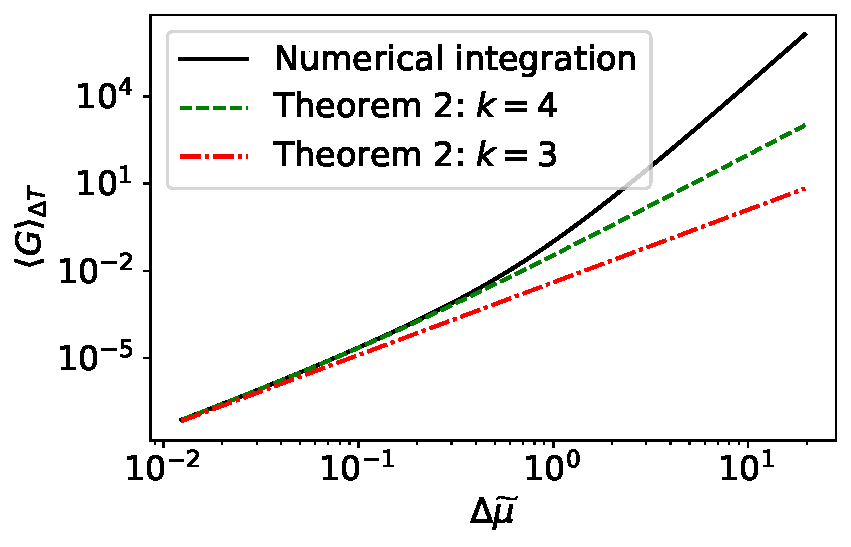
\includegraphics[width=0.49\textwidth]{./plot/FD_avg_expansion_comparison_T_decay_faster.pdf}
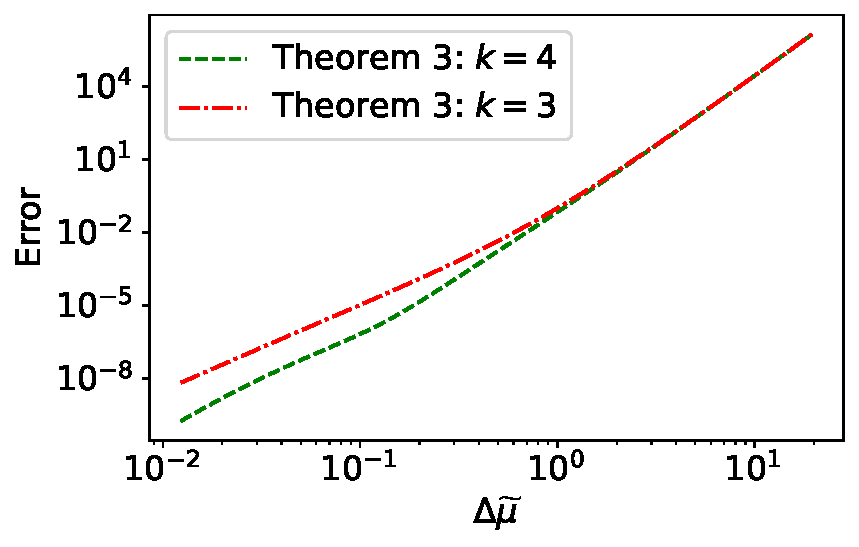
\includegraphics[width=0.49\textwidth]{./plot/FD_avg_expansion_error_comparison_T_decay_faster.pdf}
\caption{Comparison of the computation of $\langle G\rangle_{\Delta T}$   (left) using the expansion \eqref{eq:asymp_FD_int_b_decay} for $m=1.5$, $\gamma=1/2$, $d=1$, and $G(p)=(m+p)/E$, with the result obtained via numerical integration of \eqref{eq:T_faster_orig_integral}. The right plot shows the difference between the numerical result and the expansion \eqref{eq:T_faster_expansion_final} corresponding to $k=2$ and $k=3$ (note that no terms are present at $k=1$ in this case as the leading term scales with $\Delta\widetilde{\mu}^{5/2}$).  The right plot shows the difference between the numerical result and the two expansions.  On a log-log plot  the slopes can be measured to be approximately $7/2$ and $3$, correctly matching the indicated order of the expansion error in $\Delta\widetilde{\mu}$. }\label{fig:T_faster_expansion_comparison}
\end{figure}


\section{Asymptotic Expansion of Thermal Averages as $T\to 0$ with $\mu=m+\mathcal{O}(T)$}\label{sec:asympt_Delta_mu_order_T}
The decomposition of the FD distribution presented above is not as useful for studying the regime where $\mu$ approaches to $m$ as fast or faster than $T$ approaches to $0$.  This can be motivated by noting that the zero temperature contribution  is defined with respect to a fixed $\mu$ and this choice makes little sense  in the regime where $\mu=m+\mathcal{O}(T)$.  In this appendix we show that an asymptotic expansion as $T\to 0$ in this regime is more easily obtained by using the FD distribution as a whole, in contrast to the cases studied in Sections  \ref{sec:asymp_T_0_faster} and \ref{Section:HighTempSommerfeld}.


  Here we consider a $D$-dimensional thermal average ($D\geq 2$) of a function   $G(p)$, $p\in[0,\infty)$ that is a $C^k$ function whose zeroth through $k$'th derivatives are polynomially bounded and will assume that $\mu=m+bT$ where $b\geq 0$. First change variables to $z=(E-m)/m$ so that $p=m\sqrt{z}\sqrt{z+2}$
\begin{align}
&\int_0^\infty dp\, p^{D-1} G(p) f_{FD}(p)\notag\\
=&m^{D}\int_0^\infty dz\, (1+z) z^{(D-2)/2} (z+2)^{(D-2)/2} G\left(m\sqrt{z}\sqrt{z+2}\right) \frac{1}{1+e^{z/\widetilde{T}-b}}\,,\label{eq:fd_int_var_z}
\end{align}
where $\widetilde{T}\equiv T/m$.  Note that the integrand can have a square root singularity at $z=0$ and so we cannot simply Taylor expand in $z$.  However we can employ a more general asymptotic expansion  by again making use of the function $F(y,m)$, defined in \eqref{eq:F_y_m_def}, and its expansion \eqref{eq:F_y_m_Taylor}, to rewrite the integral as follows:
\begin{align}
    \eqref{eq:fd_int_var_z}=&m^{D}\int_0^\infty dz\, F(\sqrt{z},m)\frac{z^{(D-2)/2}}{1+e^{z/\widetilde{T}-b}}\\
    =&\sum_{n=0}^{k-1} a_n(m)m^{D}\int_0^\infty dz\,  \frac{z^{(n+D-2)/2}}{1+e^{z/\widetilde{T}-b}}+m^{D}\int_0^\infty dz\, R_k(\sqrt{z},m)\frac{z^{(D-2)/2}}{1+e^{z/\widetilde{T}-b}}\,.\notag
\end{align}
The remainder term can be bounded as follows
\begin{align}
 &\left|m^{D}\int_0^\infty dz\, R_k(\sqrt{z},m)\frac{z^{(D-2)/2}}{1+e^{z/\widetilde{T}-b}}\right|\\
 \leq&m^{D}\int_0^\infty dz\, [\alpha_k(m)+\beta_k(m)z^{q_k/2}]\frac{z^{(k+D-2)/2}}{1+e^{z/\widetilde{T}-b}}\notag\\
 \leq &m^{D}\int_{b\widetilde{T}}^\infty dz\, [\alpha_k(m)+\beta_k(m)z^{q_k/2}]z^{(k+D-2)/2}e^{-z/\widetilde{T}+b}\notag\\
 &+m^{D}\int_0^{{b\widetilde{T}}} dz\, [\alpha_k(m)+\beta_k(m)z^{q_k/2}]z^{(k+D-2)/2}\notag\\
 =&m^{D} \alpha_k(m)\widetilde{T}^{(k+D)/2}\int_{0}^\infty du\,(u+b)^{(k+D-2)/2}e^{-u}\notag\\
 &+m^D\beta_k(m)\widetilde{T}^{(k+D+q_k)/2}\int_{0}^\infty du\,(u+b)^{(k+D-2+q_k)/2}e^{-u}\notag\\
 &+\alpha_k(m)m^{D}\frac{2}{k+D}(b\widetilde{T})^{(k+D)/2}+\beta_k(m)m^{D}\frac{2}{k+D+q_k}(b\widetilde{T})^{(k+D+q_k)/2}\notag\\
 =&\mathcal{O}(\widetilde{T}^{(k+D)/2})\,.\label{eq:combined_exp_remainder}
\end{align}
\begin{remark}\label{remark:combined_remainder_uniform_in_b}
We emphasize that the implied constant in the bound \eqref{eq:combined_exp_remainder} depends on $m$ and $b$, though if one restricts $b$ to a bounded set then the constant can be chosen independent of $b$. 
\end{remark}

Changing variables to $x=z/\widetilde{T}$, recalling the integral formula for the polylogarithm function $\mathrm{Li}_s(y)$, see 3.411.3 in  \cite{Gradshteyn:1943cpj}:
\begin{align}\label{eq:h_decomp_eval}
   \int_0^\infty dx \, \frac{x^{n/2}}{1+e^{x-b}}    =-\Gamma(1+n/2)\mathrm{Li}_{1+n/2}(-e^b)\,,
\end{align}
and using the  remainder bound \eqref{eq:combined_exp_remainder} we obtain the following asymptotic expansion.
\begin{theorem}\label{thm:asymp_FD_int_Delta_mu_small}
Let $D\geq 0$, $k\in\mathbb{Z}^+$, and $G(p)$ be a  $C^k$ function on $[0,\infty)$ whose zeroth through $k$'th derivatives are polynomially bounded.  Let $\mu=m+bT$ for $b\geq 0$. Then
\begin{align}\label{eq:asymp_FD_int}
&\int_0^\infty dp\, p^{D-1} G(p) f_{FD}(p)\notag\\
   =&\sum_{n=0}^{k-1} a_n(m)m^{D}\widetilde{T}^{(n+D)/2}\left(-\Gamma((n+D)/2)\mathrm{Li}_{(n+D)/2}(-e^b)\right)+\mathcal{O}(\widetilde{T}^{(k+D)/2})\,,
\end{align}
where $\widetilde{T}=T/m$, $a_n$ is defined in \eqref{eq:an_def}, and the implied constant in the error term depends on $m$ but is uniform in $b$ when restricted to a fixed bounded set. 
\end{theorem}
Explicit formulas for the first few $a_n$'s can be found in Eq.~\eqref{eq:first_few_a_ns}.
\subsection{Asymptotic Expansion in the Regime $T\ll m$, $\mu=m$}\label{sec:b_0}
When $b=0$ (i.e., $\mu=m$) one can use the integral formula \eqref{eq:FD_power_integrals} to further simplify the expansion \eqref{eq:asymp_FD_int}:
\begin{align}\label{eq:asymp_FD_int_b_0}
&\int_0^\infty dp\, p^{D-1} G(p) f_{FD}(p)\notag\\
   =&\sum_{n=0}^{k-1} a_n(m)m^{D}\widetilde{T}^{(n+D)/2}(1-2^{-(n+D-2)/2})\Gamma((n+D)/2)\zeta((n+D)/2)\\
   &+\mathcal{O}(\widetilde{T}^{(k+D)/2})\,.\notag
\end{align}
In particular, note that when $D=3$ and $G(0)\neq 0$ the leading order term scales with $\widetilde{T}^{3/2}$.  This is in contrast to the  Sommerfeld expansion (see Eq. (58.1) on page 170 of \cite{landau2013statistical}), which  applies to the case where $\mu-m$ is bounded away from zero and whose leading order term scales with $\widetilde{T}^2$.




\subsection{Asymptotic Expansion in the Regime $\mu-m\ll T\ll m$}\label{sec:decaying_b}
One can also use the expansion \eqref{eq:asymp_FD_int} to study the regime where $\mu$ approaches $m$ faster than $T$ approaches zero. Mathematically we parameterize this as 
\begin{align}\label{eq:mu_decay_faster}
\mu=m(1+B\widetilde{T}^{1+\gamma})\,,\,\,\,  B\geq 0\,,\,\, \gamma>0\,.   
\end{align}
  To proceed, first  Taylor expand \eqref{eq:h_decomp_eval} by differentiating under the integral to obtain
\begin{align}\label{eq:Li_expansion}
    &-\Gamma(1+n/2)\mathrm{Li}_{1+n/2}(-e^b)\\
    =&\int_0^\infty du \, \frac{u^{n/2}}{1+e^{u-b}}    \notag\\
    =&\int_0^\infty du\,\frac{u^{n/2}}{e^u+1}+b\int_0^\infty du\,\frac{u^{n/2}}{(e^{u/2}+e^{-u/2})^2}  +\mathcal{O}(b^2)\notag\\
    =&(1 - 2^{-n/2}) \Gamma(1 + n/2) \zeta(1 + n/2)+ b\int_0^\infty du\,\frac{u^{n/2}}{(e^{u/2}+e^{-u/2})^2} +\mathcal{O}(b^2)\,.\notag
\end{align}
For $n=0$ the leading order term in the above expression has the indeterminant form $0\cdot \infty$ (this case will only be  relevant to us when $D=2)$; there one should instead use
\begin{align}
\int_0^\infty du \frac{1}{1+e^{u-b}}=\ln(1+e^b)=    \ln(2)+\frac{b}{2}+\mathcal{O}(b^2)\,.
\end{align}
Now substitute \eqref{eq:Li_expansion} into \eqref{eq:asymp_FD_int} and let $b=B\widetilde{T}^\gamma$ (we note that the remainder term in \eqref{eq:asymp_FD_int} is still $\mathcal{O}(\widetilde{T}^{1+(k+D-2)/2})$ in this case because $b$ remains bounded as $\widetilde{T}\to 0$; see Remark \ref{remark:combined_remainder_uniform_in_b}). Assuming $\gamma\geq 1/2$  the expansion \eqref{eq:asymp_FD_int} with $k=2$ simplifies to give the following result.
\begin{theorem}\label{thm:mu_zero_faster}
Let $G(p)$ be a $C^2$ function on $[0,\infty)$ whose zeroth through $2$nd derivatives are polynomially bounded.  Let $\mu=m(1+B\widetilde{T}^{1+\gamma})$, $B\geq 0$, $\gamma\geq 1/2$. 
\begin{enumerate}
    \item For $D=3$ we have
    \begin{align}
&\int_0^\infty dp\, p^{2} G(p) f_{FD}(p)\label{eq:FD_b_decay_orig_integral}\\
   =&a_0(m)m^{3}(1 - 2^{-1/2}) \frac{\pi^{1/2}}{2} \zeta(3/2)\widetilde{T}^{3/2}+  \frac{\pi^2}{12}a_1(m)m^{3}\widetilde{T}^{2}\label{eq:asymp_FD_int_b_decay}\\
   &+ Ba_0(m)m^{3}\widetilde{T}^{\gamma+3/2}\int_0^\infty du\,\frac{u^{1/2}}{(e^{u/2}+e^{-u/2})^2} 
   +\mathcal{O}(\widetilde{T}^{5/2})\notag
\end{align}
as $T\to 0$, where $\widetilde{T}=T/m$ and $a_n$ is defined by \eqref{eq:an_def} with $D=3$.
\item For $D=2$ we have
\begin{align}
&\int_0^\infty dp\, p G(p) f_{FD}(p)\\
   =& a_0(m)m^{2}\ln(2)\widetilde{T}
+\frac{1}{2}Ba_0(m)m^{2}\widetilde{T}^{1+\gamma}\\
   &+ a_1(m)m^{2}
 (1 - 2^{-1/2}) \frac{\pi^{1/2}}{2} \zeta(3/2)\widetilde{T}^{3/2}+ 
   \mathcal{O}(\widetilde{T}^{2})\,,\notag
\end{align}
as $T\to 0$, where $\widetilde{T}=T/m$ and $a_n$ is defined by \eqref{eq:an_def} with $D=2$.
\end{enumerate}
\end{theorem}
\begin{remark}
 When referring to the number of terms in the expansions in Theorem \ref{thm:mu_zero_faster} and related results, e.g., in \ref{fig:FD_avg_expansion_comparison_Sommerfeld},  we mean the index $k$ that was used in \eqref{eq:asymp_FD_int} to obtain the expansion.
\end{remark}
To obtain higher order terms in  Theorem \ref{thm:mu_zero_faster}, or to consider  $\gamma<1/2$ or $D\neq 2,3$, one simply needs to  continue the expansion \eqref{eq:Li_expansion} to the appropriate higher order before substituting it into \eqref{eq:asymp_FD_int}; however, we again emphasize that these results are asymptotic expansions and so going to higher order does not necessarily increase the accuracy at a given $T$. We note that the integral over $u$ appearing in \eqref{eq:asymp_FD_int_b_decay} does not depend on the values of the parameters and is of a form that can be  reliably approximated via standard numerical quadrature.  In Figure \ref{fig:FD_avg_expansion_comparison_Sommerfeld} we show a comparison between the expansion \eqref{eq:asymp_FD_int_b_decay} (green dashed line) and numerical integration of \eqref{eq:FD_b_decay_orig_integral} (solid black line).  We also compare with the Sommerfeld expansion \eqref{} (red dot-dashed line).  Note that the Sommerfeld completely fails in the low temperature regime when $\mu$ and $T$ are related by \eqref{eq:mu_decay_faster} (i.e., when $\mu-m\ll T$).  Under the parameterization \eqref{eq:mu_decay_faster}, the classical Sommerfeld expansion is actually seen to be valid at high temperature; we prove this to be the case in Theorem \ref{thm:high_T_Sommerfeld}.

\begin{figure}
\centering
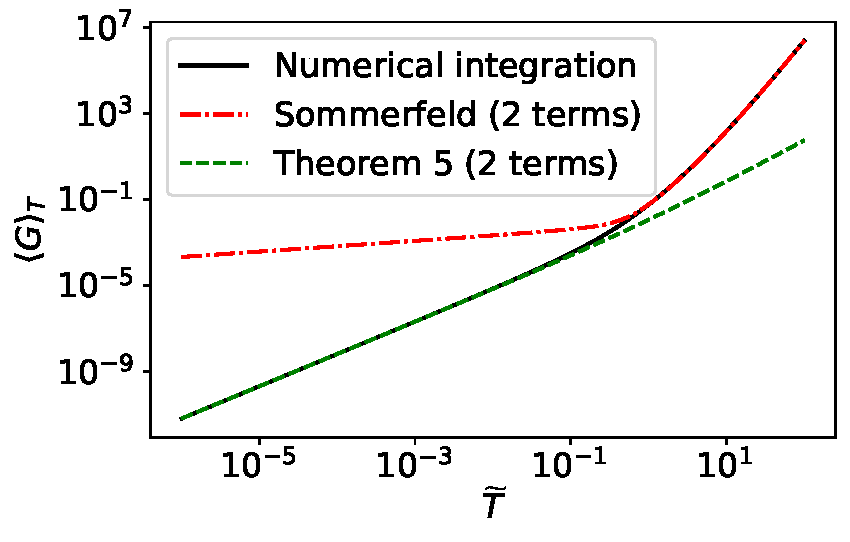
\includegraphics[width=0.49\textwidth]{./plot/Sommerfeld_high_temp_comparison.pdf}
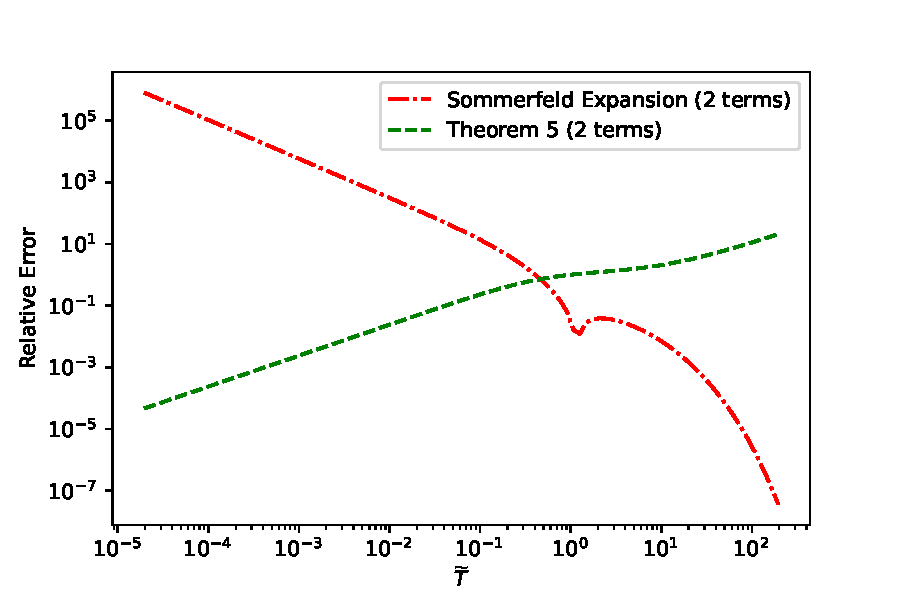
\includegraphics[width=0.49\textwidth]{./plot/Sommerfeld_high_temp_relative_error_comparison.pdf}
\caption{Left: Comparison of asymptotic expansions of $\langle G\rangle_{\Delta T}$, $G(p)=1$, via the Sommerfeld expansion \eqref{eq:Sommerfeld_high_temp_final} (red dot-dashed line) and the new expansion  \eqref{eq:asymp_FD_int_b_decay}  (green dashed  line) where  $\mu=m(1+\widetilde{T}^{3/2})$.  Under this relationship between $\mu$ and $T$, Theorem \ref{thm:high_T_Sommerfeld} and Theorem \ref{thm:mu_zero_faster} respectively prove that \eqref{eq:Sommerfeld_high_temp_final} is valid at high temperature and \eqref{eq:asymp_FD_int_b_decay} is valid at low temperature; we see this reflected in the figure. Right: The relative error of these asymptotic expansions.  }\label{fig:FD_avg_expansion_comparison_Sommerfeld}
\end{figure}





%%%%%%%%%%%%%%%%%%%%%%%%%%%%%%%%%%%%%%%
\section{Results and Discussion}
\label{sec12}
In this work, we introduce a novel form of the Fermi distribution Eq.~(\ref{NFF1}) that separates the Fermi gas into zero and finite temperature components analytically. This is the first time in literature that has clean separation of the zero and finite temperature components. Unlike the traditional brutal approach to eliminating the $T=0$ limit from the low-temperature Fermi distribution, our novel form of the Fermi distribution for finite temperature component has several numerical advantages in computation. {\xgreen The prescription proposed here is in terms of distribution rather than analytical function. However, for all physical applications it is only necessary to calculate integrals for which the exact behavior at $x=0$ is not required.}

 
The mathematical form of the finite temperature components is well-suited for numerical calculations and can be used to address the integrals common in statistical physics. This is because the finite temperature components are naturally exponentially suppressed while also preserving the sign of all corrections making the formulation easier to numerically integrate and reduce the numerical noise, see Fig.~\ref{Fermi_Component}. 


To illustrate the advantage of our novel form of distribution can be used to address the integrals common in physics, we examine the thermal average quantity $\langle G\rangle_T$ for any given function $G(p)$. The assumptions on $G(p)$ are quite modest, only requiring smoothness and polynomial growth bounds on $G$ and it's derivatives as $p\to \infty$. 


Our novel decomposition guides the asymptotic analysis of $\langle G\rangle_{\Delta T}-\langle G\rangle_\Theta$ by naturally reorganizing the integrand into a difference of integrals with exponentially decaying integrands. This allows us to utilize asymptotic analysis techniques to   extract  leading and subleading order behavior as $T\to 0$. 

The finite temperature contribution is naively written as a difference of integrals, with the leading order contribution in $T$ of the former canceling that of the latter.  This leads to instability when attempting to compute $\langle G\rangle_{\Delta T}-\langle G\rangle_\Theta$ via numerical integration for small $T$.  This issue is eliminated when using the asymptotic expansion derived below, where we are able to account for this exact cancellation analytically. 

 
The Fermi distribution Eq.~(\ref{NFF1}) provides us the tool to study or examine the effects and characteristics of finite temperature components separately. In addition, our approach also allows for analytical exploration of the finite temperature contributions by expanding the function around the Fermi-energy surface.


%{\xgreen I finished editing this section so that it is in terms of unitless quantities. It seems to me though that the $p_\mu$ scale is somewhat arbitrary...equivalently we could use $m$ or $\mu$ not sure which is better. Also, I renamed the chemical potential to $\mu$ without tilde so that I can use tilde for re-scaled quantities. M.} 
%{\bf Great, thanks.  Yes, I agree there is nothing unique about the choice and mathematically we could have chosen $\mu$ or $m$ but I do think $p_\mu$ is better since it is the combination of $m$ and $\mu$ that naturally shows up in the denominator of certain terms.  It suggests at a glance that the expansion can encounter trouble if any of $\mu/p_\mu$, $m/p_\mu$ or $T/p_\mu$ is large, even if strictly speaking the result concerns the asymptotic behavior in $T$.} {\xgreen Based on the formulas I added at the end I believe that this can be significantly simplified still. No need to explicitly state the dimension $D$ because we can absorb it to arbitrary function $G(p)$. Also, we can start with the integral over $dE H(E) f_{FD}(E)$ from the beginning which saves one switch of variables and at the end we get an expression which is more useful for calculating some standard thermodynamical properties....like heat capacity. See also equation 58.1 in Landau-Lifshitz \url{https://www.charmille.art/books/Landau_Lifshitz_T5.pdf}}



%%%%%%%%%%%%%%%%%%%%%%%%%%%%%%%%%%%%%%%
%%%%%%%%%%%%%%%%%%%%%%%%%%%%%%%%%%%%%%%%%%%
%%%%%%%%%%%%%%%%%%%%%%%%%%%%%%%%%%%%%%%


\appendix






\section{Sommerfeld Expansion in the Regime $\mu\gg T\gg m$}\label{Section:HighTempSommerfeld}
The classical Sommerfeld expansion can also be extended to an appropriate high temperature regime, with $\mu$ growing faster than $T$.  Specifically, we paramaterize $\mu$ as a function of $T$ as follows
\begin{align}\label{eq:mu_infinity_faster}
\mu=m(1+B\widetilde{T}^{1+\gamma}) \,,\,\,\gamma,B>0\,.   
\end{align}
Note that this is the same functional relation as considered in Section \ref{sec:decaying_b} but here we study the high-temperature limit.  We will assume that the density of states $H(E)$ is continuous on $[m,\infty)$ and is smooth on a neighborhood of $\infty$ and we have an odd $k>1$ such that the $k$'th derivative of $H$ the following asymptotic behavior as $E\to\infty$ for some $a_k\neq 0$, $q_k\in\mathbb{R}$:
\begin{align}\label{eq:H_deriv_asymp}
    H^{(k)}(E)=a_kE^{q_k}+ \mathcal{O}(E^{q_k-1})\,.
\end{align}
By integrating this expression and combining it with the assumption that $H$ is continuous we can conclude that $H$ is also polynomially bounded on $[m,\infty)$. We note that, by definition, the asymptotic behavior \eqref{eq:H_deriv_asymp} implies that there exists $E_0$ and $C$ such that $H$ is smooth on $[E_0,\infty)$ and $|H^{(k)}(E)-a_kE^{q_k}|\leq CE^{q_k-1}$ for all $E\in[E_0,\infty)$. For the remainder of this derivation we assume that $T$ is large enough to ensure $\mu\geq E_0$. 

Now use  the decomposition \eqref{Eq_form} to write
\begin{align}
    &\int_m^\infty dE\, H(E)(f_{T\neq 0}+\widetilde{f}_{T\neq 0})\notag\\
    =&\int_\mu^\infty dE \,H(E)\frac{1}{1+e^{(E-\mu)/T}}-\int_m^\mu dE\, H(E)\frac{1}{1+e^{(\mu-E)/T}}\notag\\
=&T\int_0^\infty dz \,H(\mu+Tz)\frac{1}{1+e^{z}}-T\int^{(\mu-m)/T}_0 dz\, H(\mu-Tz)\frac{1}{1+e^{z}}\,,\label{eq:Sommerfeld_high_temp_z}
\end{align}
where we changed variables to $z=(E-\mu)/T$ in the first integral and $z=(\mu-E)/T$ in the second.  Due to the exponentially decaying factor in the integrands in \eqref{eq:Sommerfeld_high_temp_z} along with polynomial boundedness of $H$, we can shrink the upper limits of integration  to $(\mu-E_0)/T$, thereby ensuring that $\mu-Tz\geq E_0$ on the domain of integration, with the  error incurred by this change being $\mathcal{O}(T^{-p})$ as $T\to \infty$ for any choice of $p>0$; this which will be negligible compared to the other asymptotic approximations made below.  With this we can write
\begin{align}
    &\int_m^\infty dE\, H(E)(f_{T\neq 0}+\widetilde{f}_{T\neq 0})\notag\\
=&T\int_0^{\frac{\mu-E_0}{T}} dz \,\frac{H(\mu+Tz)- H(\mu-Tz)}{1+e^{z}}+\mathcal{O}(T^{-p})\,. \label{eq:Sommerfeld_high_temp_z2}
\end{align}
As $\mu\pm Tz\geq E_0$ for all $z$ in the domain of integration, we can compute a Taylor expansion with remainder up to order $k$ as follows:
\begin{align}
 &H(\mu+Tz)- H(\mu-Tz)=\sum_{n=1,n\text{ odd}}^{k-2} 2H^{(n)}(\mu)\frac{(Tz)^n}{n!}\\
 &\qquad\qquad\qquad+(Tz)^k \int_0^1 ds\,\frac{(1-s)^{k-1}}{(k-1)!} (H^{(k)}(\mu+sTz)+H^{(k)}(\mu-sTz))\,. \notag
\end{align}
Substituting this into \eqref{eq:Sommerfeld_high_temp_z2} and again making use of the freedom to change the limits of integration while only incurring $\mathcal{O}(T^{-p})$ error and using the integral formulas \eqref{eq:FD_power_integrals} we find
\begin{align}
    &\int_m^\infty dE\, H(E)(f_{T\neq 0}+\widetilde{f}_{T\neq 0})\notag\\
    =&\sum_{n=1,n\text{ odd}}^{k-2} \frac{2T^{n+1}}{n!}H^{(n)}(\mu)\int_0^{\frac{\mu-E_0}{T}} dz \,\frac{z^n}{1+e^{z}}+R_k
+\mathcal{O}(T^{-p})\notag\\
=&\sum_{n=1,n\text{ odd}}^{k-2} 2(1-2^{-n})\zeta(n+1)T^{n+1}H^{(n)}(\mu)
+R_k
+\mathcal{O}(T^{-p})\,,\label{eq:Sommerfeld_high_temp_z3}
\end{align}
where the remainder term is given by
\begin{align}
    R_k\equiv T^{k+1}\int_0^{\frac{\mu-E_0}{T}} dz \,\frac{z^k}{1+e^{z}}
 \int_0^1 ds\, \frac{(1-s)^{k-1}}{(k-1)!} (H^{(k)}(\mu+sTz)+H^{(k)}(\mu-sTz))\,.
\end{align}
Eq.~\eqref{eq:H_deriv_asymp} implies that $|H^{(k)}(E)|\leq CE^{q_k}$ on $[E_0,\infty)$ for some $C>0$. Using this we can bound the remainder as follows:
\begin{align}
    |R_k|\leq &CT^{k+1}\int_0^{\frac{\mu-E_0}{T}} dz \,\frac{z^k}{1+e^{z}}
 \int_0^1 ds\, \frac{(1-s)^{k-1}}{(k-1)!} \left(|\mu+sTz|^{q_z}+|\mu-sTz|^{q_k}\right)\notag\\
 \leq&2^{q_k+1}CT^{k+1}\int_0^{\infty} dz \,\frac{z^k}{1+e^{z}}\notag
 \int_0^1 ds\, \frac{(1-s)^{k-1}}{(k-1)!} (\mu^{q_k}+(sTz)^{q_k})\notag\\
 =&\mathcal{O}(\mu^{q_k}T^{k+1})\label{eq:Sommerfeld_high_T_remainder_bound}
\end{align}
as $T\to\infty$.  Note that due to the  relation \eqref{eq:mu_infinity_faster} between $\mu$ and $T$ we can equivalently write the error term as $\mathcal{O}(T^{(1+\gamma)q_k+k+1})$ and so the $\mathcal{O}(T^{-p})$ error term is negligible in comparison. Combining the above remainder bound with \eqref{eq:Sommerfeld_high_temp_z3} we obtain the following asymptotic expansion.
\begin{theorem}\label{thm:high_T_Sommerfeld}
Let $k\in\mathbb{Z}^+$ be odd and suppose that $H(E)$ is continuous on $[m,\infty)$, is smooth on a neighborhood of $\infty$, and
\begin{align}
  H^{(k)}(E)=a_kE^{q_k}+\mathcal{O}(E^{q_k-1})  
\end{align}
as $E\to \infty$ for some $a_k\neq 0$, $q_k\in\mathbb{R}$.  Let $\mu=m(1+B\widetilde{T}^{1+\gamma})$, $\gamma,B>0$, $\widetilde{T}\equiv T/m$. Then
\begin{align}
    &\int_m^\infty dE\, H(E)f_{FD}(E)\notag\\
=&\int_m^\mu dE\, H(E)+\sum_{n=1,n\text{ odd}}^{k-2} 2(1-2^{-n})\zeta(n+1)T^{n+1}H^{(n)}(\mu)+\mathcal{O}(\mu^{q_k}T^{k+1})\label{eq:Sommerfeld_high_temp_final}
\end{align}
as $T\to\infty$.
\end{theorem}
When $q_k>0$ the absolute error in \eqref{thm:high_T_Sommerfeld}  grows as $T\to\infty$ but the relative error decays, as we now show.  First, integrate \eqref{eq:H_deriv_asymp} twice to get
\begin{align}\label{eq:integrate_H_asymp}
    H^{(k-2)}(\mu)=\frac{a_k}{(q_k+1)(q_k+2)}\mu^{q_k+2}+\mathcal{O}(\mu^{q_k+1})
\end{align}
as $\mu\to\infty$, assuming $q_k>0$; we do not consider these cases further here). Therefore, the ratio of the error to the last included term in the expansion behaves as
\begin{align}\label{eq:Sommerfeld_high_T_rel_err}
&\frac{\mathcal{O}(\mu^{q_k}T^{k+1})}{ T^{k-1} H^{(k-2)}(\mu)}=\frac{T^2}{\mu^2}\frac{\mathcal{O}(1)}{ \frac{a_k}{(q_k+1)(q_k+2)}+\mathcal{O}(\mu^{-1})}= \mathcal{O}(T^{-2\gamma})\,,
\end{align}
where we used \eqref{eq:mu_infinity_faster} and also that $a_k\neq 0$. Continuing to integrate \eqref{eq:integrate_H_asymp}, one sees that earlier terms in the sum dominate the error term to a  greater degree.  Therefore the expansion \eqref{eq:Sommerfeld_high_temp_final} properly  captures leading and sub-leading behavior, with a subdominant error term and a decaying relative error when $q_k>0$. When $q_k\leq 0$, integrating \eqref{eq:H_deriv_asymp} becomes more subtle due to the need to handle potential logarithm and constant terms that arise.  However, if instead we make the additional assumptions 
\begin{align}
H^{(k-j)}(E)=a_{k-j} E^{q_k+j} +\mathcal{O}(E^{q_k+j-1})
\end{align}
for $j=2,...,k-1$ with $a_{k-j}\neq 0$ then a similar computation to \eqref{eq:Sommerfeld_high_T_rel_err} shows
\begin{align}
    \frac{\mathcal{O}(\mu^{q_k}T^{k+1})}{T^{n+1}H^{(n)}(\mu)}= \mathcal{O}(T^{-(k-n)\gamma})
\end{align}
for all $n=1,...,k-2$ and therefore the error term in \eqref{eq:Sommerfeld_high_temp_final} is again seen to be dominated by all other terms in the summation as $T\to\infty$. In Figure \ref{fig:FD_avg_expansion_comparison_Sommerfeld} we present a  numerical demonstration of the validity of \eqref{eq:Sommerfeld_high_temp_final} in the high temperature regime. In   Figure \ref{fig:Thm3_vs_Sommerfeld_regions_terms_comp} we plot the domain of validity of the  Sommerfeld expansion  and compare it with that of the expansion from Theorem \ref{thm:mu_zero_faster}.  In particular, we note that the domain of validity when using 2 terms (right) of the Sommerfeld expansion is reduced in many areas, as compared to the region for 1 term (left). This is typical of results such as Theorem \ref{thm:high_T_Sommerfeld} that give asymptotic, but not convergent, expansions.




\begin{figure}
\centering
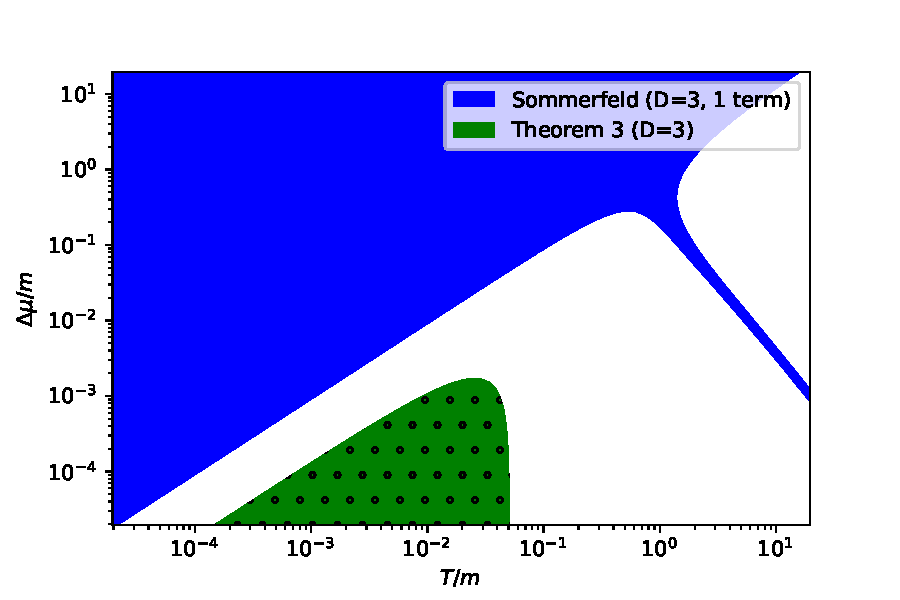
\includegraphics[width=0.49\textwidth]{./plot/Sommerfeld_vs_Thm3_regions_D3_1_term.pdf}
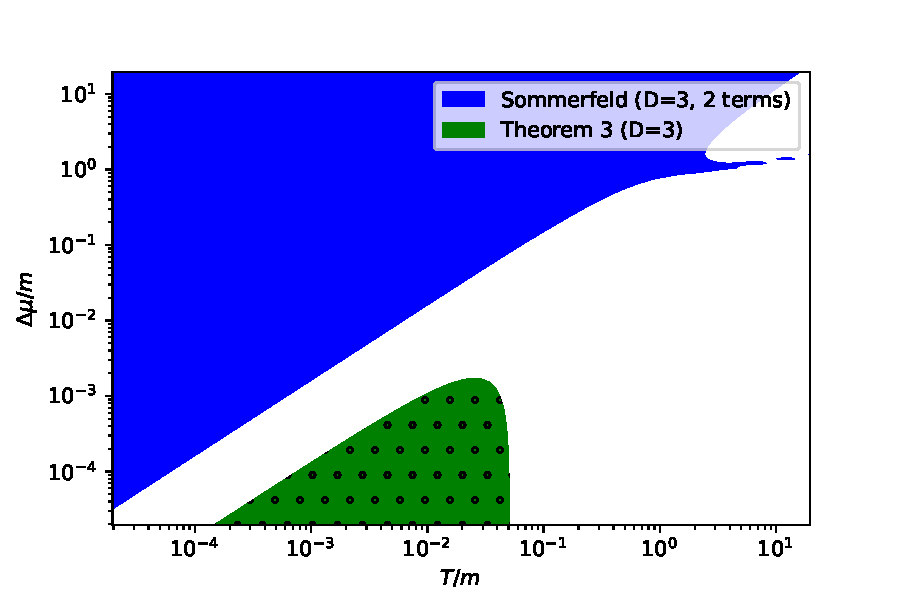
\includegraphics[width=0.49\textwidth]{./plot/Sommerfeld_vs_Thm3_regions_D3_2_terms.pdf}
\caption{Domains of validity for $D=3$ in $(T/m,\Delta\mu/m)$-space ($\Delta\mu\equiv\mu-m$) of the Sommerfeld expansion (solid blue) and the expansion from Theorem \ref{thm:mu_zero_faster} (dotted green), where validity is defined as the computation of $\langle G\rangle_T$ having relative error  less that $10\%$ for the choice  $G(p)=1$.  Our new expansion from Theorem \ref{thm:mu_zero_faster} applies when $\Delta\mu\ll T\ll m$.  Note that in addition to the well-known low temperature regime, there is also a high-temperature regime ($\mu\gg T\gg m$) where the Sommerfeld expansion is also valid, as proven in Theorem \ref{thm:high_T_Sommerfeld}. }\label{fig:Thm3_vs_Sommerfeld_regions_terms_comp}
\end{figure}

%%%%%%%%%%%%%%%%%%%%%%%%%%%%%%%%%%%%%%%

\backmatter

\bmhead{Acknowledgments}
We thank Gordon Baym and John W. Clark for their encouragement to pursue research into this novel form of the Fermi distribution which lead to this work.

%%%%%%%%%%%%%%%%%%%%%%%%%%%%%%%%%%%%%%%
\bibliography{novel-fermi-function-refs}
%% if required, the content of .bbl file can be included here once bbl is generated
%%\input sn-article.bbl
\end{document}







%%%%%%%%%%%%%%%%%%%%%%%%%%%%%%%%%%%%

\section{Old Version: Asymptotic Expansion of Thermal Averages as $T\to 0$ with $\mu=m+\mathcal{O}(T)$}
{\bf ?? To be removed in final??}

In this section we use the decomposition \eqref{Eq_form} to obtain an asymptotic expansion for the difference between a $D$-dimensional thermal average ($D\geq 2$) at finite and zero temperature as $T\to 0$ and when $\mu=m+\mathcal{O}(T)$.   More specifically, we will assume that $\mu=m+bT$ where $b\geq 0$ and that $G(p)$, $p\in[0,\infty)$, is a $C^k$ function whose zeroth through $k$'th derivatives are polynomially bounded.

Start by changing variables to $E=\sqrt{p^2+m^2}$:
\begin{align}
    &\int_0^\infty dp\, p^{D-1} G(p)(f_{T\neq 0}+\widetilde{f}_{T\neq 0})\notag\\
=&\int_0^\infty dp\, p^{D-1} G(p)\frac{1}{2}e^{-|E-\mu|/T}\left\{\mathrm{sgn}(E-\mu)+\tanh[(E-\mu)/(2T)]\right\}\notag\\
    =&\int_m^\infty dE \,Ep^{D-2} G\left(\sqrt{E^2-m^2}\right)\frac{1}{2}e^{-|E-\mu|/T}\left\{\mathrm{sgn}(E-\mu)+\tanh[(E-\mu)/(2T)]\right\}\notag\\
    =&\int_{\mu}^\infty dE\, E(E^2-m^2)^{(D-2)/2} G\left(\sqrt{E^2-m^2}\right)
    \frac{1}{1+e^{(E-\mu)/T}}\label{eq:2_int_decomp}  \\
    &-\int_m^{\mu} dE \,E(E^2-m^2)^{(D-2)/2} G\left(\sqrt{E^2-m^2}\right)\frac{1}{1+e^{(\mu-E)/T}} \,.\notag
\end{align}
Now consider the first integral in \eqref{eq:2_int_decomp}. Changing variables to $z=(E-m)/m$ gives
\begin{align}\label{eq:int_1_change_vars}
&\int_{\mu}^\infty dE\, E(E^2-m^2)^{(D-2)/2} G\left(\sqrt{E^2-m^2}\right)
    \frac{1}{1+e^{(E-\mu)/T}}   \\
    =&m^{D}\int_{b\widetilde{T}}^\infty dz\, (z+1)[(z+1)^2-1]^{(D-2)/2} G\left(m\sqrt{(z+1)^2-1}\right)
    \frac{1}{1+e^{z/\widetilde{T}-b}}\notag\\
        =&m^{D}\int_{b\widetilde{T}}^\infty dz\, (z+1)z^{(D-2)/2}(z+2)^{(D-2)/2} G\left(m\sqrt{z}\sqrt{z+2}\right)
    \frac{1}{1+e^{z/\widetilde{T}-b}}\,,\notag
\end{align}
where $\widetilde{T}\equiv T/m$.  Note that the lower limit of integration approaches $0$ in the regime under consideration and that, in general, the integrand has a singularity there.  Thus is is important that we not simply assume the integrand is smooth and has a Taylor expansion; a more general asymptotic expansion is needed. 
\begin{comment}
    To accomplish this, define
\begin{align}\label{eq:F_y_m_def}
    F(y,m)\equiv(y^2+1)(y^2+2)^{(D-2)/2}G\left(my\sqrt{y^2+2}\right)\,.
\end{align}
We have assumed that $G$ is $C^k$ on $[0,\infty)$ with polynomially bounded zeroth through $k$'th derivatives and therefore $y\mapsto F(y,m)$ also has these properties.  We can therefore use Taylor's theorem with remainder to write
\begin{align}\label{eq:F_y_m_Taylor}
F(y,m)=&\sum_{n=0}^{k-1} a_n(m)y^n +R_k(y,m)\,, \,\,\,a_n(m)=\frac{1}{n!}\partial_y^n F(0,m)\,,
\end{align}
where the remainder term is given by
\begin{align}
R_k(y,m)=y^k \int_0^1\frac{(1-s)^{k-1}}{(k-1)!}\partial_y^k F(sy,m)ds
\end{align}
and can be bounded via
\begin{align}
|R_k(y,m)|\leq y^k[\alpha_k(m)+\beta_k(m)y^{q_k}]
\end{align}
for some coefficients $\alpha_k,\beta_k$ and power $q_k$.
\end{comment}

We can again make use of the function $F(y,m)$, defined in \eqref{eq:F_y_m_def}, and its expansion \eqref{eq:F_y_m_Taylor}, to rewrite the integral as
\begin{align}
   \eqref{eq:int_1_change_vars} =&m^{D}\int_{b\widetilde{T}}^\infty dz\, z^{(D-2)/2} F\left(\sqrt{z},m\right)\frac{1}{1+e^{z/\widetilde{T}-b}}\notag\\
    =&\sum_{n=0}^{k-1} a_n(m)m^{D}\int_{b\widetilde{T}}^\infty dz\, \frac{ z^{(n+D-2)/2} }{1+e^{z/\widetilde{T}-b}} +m^{D}\int_{b\widetilde{T}}^\infty dz\,   R_k\left(\sqrt{z},m\right)\frac{z^{(D-2)/2}}{1+e^{z/\widetilde{T}-b}}\notag\\   
        =&\sum_{n=0}^{k-1} a_n(m)m^{D}\widetilde{T}^{1+(n+D-2)/2}\int_{0}^\infty dx\, \frac{ (x+b)^{(n+D-2)/2} }{1+e^{x}}  \label{eq:second_int_exp_final}\\
        &+m^{D}\int_{b\widetilde{T}}^\infty dz\,   R_k\left(\sqrt{z},m\right)\frac{z^{(D-2)/2}}{1+e^{z/\widetilde{T}-b}}\,,  \notag
\end{align}
where we changed variables to $x =z/\wt{T} - b = (E-\mu)/T$ in the first $k$ terms. Making use of the bound   \eqref{eq:R_k_poly_bound}, the integral of the remainder term can be bounded as follows:
\begin{align}
 &\left|m^{D}\int_{b\widetilde{T}}^\infty dz\, R_k\left(\sqrt{z},m\right)\frac{z^{(D-2)/2}}{1+e^{z/\widetilde{T}-b}}\right|\notag\\
 \leq&m^{D}\int_{b\widetilde{T}}^\infty dz\, z^{(k+D-2)/2}[\alpha_k(m)+\beta_k(m)z^{q_k/2}]e^{-z/\widetilde{T}+b}\notag\\
 =&m^{D}\alpha_k(m)\widetilde{T}^{1+(k+D-2)/2} \int_{0}^\infty dx \,(x+b)^{(k+D-2)/2}e^{-x}\notag\\
 &+m^{D}\beta_k(m)\widetilde{T}^{1+(k+D-2+q_k)/2}\int_{0}^\infty dx\,(x+b)^{(k+D-2+q_k)/2}e^{-x}\notag\\
 =&O\left(\widetilde{T}^{(k+D)/2}\right) \,\, \text{ as }\,\widetilde{T}\to 0 \,, \label{eq:int_1_remainder_bound}
\end{align}
which is higher order in $\widetilde{T}$ than the first $k$ terms in the expansion \eqref{eq:second_int_exp_final}.
\begin{remark}\label{remark:uniform_in_b}
We emphasize that the implied constant in the bound \eqref{eq:int_1_remainder_bound} depends on $m$ and $b$, though if one restricts $b$ to a bounded set then the constant can be chosen independent of $b$. This point will be important in Section \ref{sec:decaying_b} where we consider the case of $b$ approaching $0$ as $\widetilde{T}$ does. 
\end{remark}


We use the following notation for the integrals appearing in the expansion \eqref{eq:second_int_exp_final} 
\begin{align}\label{eq:h_n_def}
    h_n(b)\equiv \int_{0}^\infty dx \,\frac{(x+b)^{n/2}}{1+e^{x}}
\end{align}
For $b=0$ they can be evaluated using, e.g.,  3.411.3 on page 353 of  \cite{Gradshteyn:1943cpj}
\begin{align}\label{eq:h_n_0}
    h_n(0)=(1-2^{-n/2})\Gamma(1+n/2)\zeta(1+n/2)\,.
\end{align}
When $b>0$ it will be useful to change variables to $u=x+b$ and decompose them as follows:
\begin{align}\label{eq:h_n_decomp}
  h_n(b)=&\int_b^\infty du\,  \frac{u^{n/2}}{1+e^{u-b}}\\
  =&\int_0^\infty du \, \frac{u^{n/2}}{1+e^{u-b}}-b^{1+n/2}\int_0^1 dw \, \frac{w^{n/2}}{1+e^{b(w-1)}}\,,\notag
\end{align}
where  $w = u/b$ and the first integral can be evaluated in terms of the polylogarithm function $\mathrm{Li}_s(x)$, see 3.411.3 in  \cite{Gradshteyn:1943cpj}:
\begin{align}\label{eq:h_decomp_eval}
   \int_0^\infty dz \, \frac{z^{n/2}}{1+e^{z-b}}    =-\Gamma(1+n/2)\mathrm{Li}_{1+n/2}(-e^b)\,.
\end{align}



Now we use these same techniques to compute an asymptotic expansion of the second integral in \eqref{eq:2_int_decomp}. Start by again changing variables  to $z=(E-m)/m$ and then  employ the Taylor expansion \eqref{eq:F_y_m_Taylor} of  the  $F(y,m)$ defined in \eqref{eq:F_y_m_def}:
\begin{align}
    &\int_m^{\mu} dE \,E(E^2-m^2)^{(D-2)/2} G\left(\sqrt{E^2-m^2}\right)\frac{1}{1+e^{(\mu-E)/T}}\\
    =&m^{D}\int_0^{b\widetilde{T}} dz  \,(1+z)z^{(D-2)/2}(z+2)^{(D-2)/2} G\left(m\sqrt{z}\sqrt{z+2}\right)\frac{1}{1+e^{b-z/\widetilde{T}}}\notag\\
    =&m^{D}\int_0^{b\widetilde{T}} dz  \,z^{(D-2)/2}F\left(\sqrt{z},m\right)\frac{1}{1+e^{b-z/\widetilde{T}}}\notag\\
        =&\sum_{n=0}^{k-1} a_n(m)m^{D}\int_0^{b\widetilde{T}} dz  \, \frac{z^{(n+D-2)/2}}{1+e^{b-z/\widetilde{T}}} +m^{D}\int_0^{b\widetilde{T}} dz\, R_k\left(\sqrt{z},m\right) \frac{z^{(D-2)/2}}{1+e^{b-z/\widetilde{T}}}\notag\\
        =&\sum_{n=0}^{k-1} a_n(m)m^{D}(b\widetilde{T})^{1+(n+D-2)/2}g_{n+D-2}(b) +m^{D}\int_0^{b\widetilde{T}} dz\, R_k\left(\sqrt{z},m\right) \frac{z^{(D-2)/2}}{1+e^{b-z/\widetilde{T}}}\,,\label{eq:int_2_expansion}\notag
\end{align}    
 where the auxiliary function $g_n(b)$ is defined as
\begin{equation}
    g_n(b)\equiv \int_0^{1} dw  \,\frac{w^{n/2} }{1+e^{b(1-w)}}\,.
\end{equation}
  One can bound the remainder term as follows
\begin{align}
 &\left|m^{D}\int_0^{b\widetilde{T}} dz\, R_k\left(\sqrt{z},m\right) \frac{z^{(D-2)/2}}{1+e^{b-z/\widetilde{T}}}\right|\\
 \leq&m^{D}\int_0^{b\widetilde{T}} dz\,   z^{(k+D-2)/2}[\alpha_k(m)+\beta_k(m)z^{q_k/2}]
 e^{-b+z/\widetilde{T}}\notag\\
 =&m^{D}e^{-b}  \widetilde{T}^{(k+D)/2} \left[\alpha_k(m)\int_0^{b} du\,u^{(k+D-2)/2} e^{u}+\beta_k(m)\widetilde{T}^{q_k/2}\!\int_0^{b} du\, u^{(k+D-2+q_k)/2} e^{u}\right]\notag\\
\leq&m^{D}  (1-e^{-b})b^{(k+D-2)/2}\widetilde{T}^{(k+D)/2}\left[\alpha_k(m) +\beta_k(m)\widetilde{T}^{q_k/2} b^{q_k/2}\right]\notag\\
=&O\left(\widetilde{T}^{(k+D)/2}\right)\,\text{ as }\, \widetilde T\to 0\,.\notag
\end{align}
Remark \ref{remark:uniform_in_b} also applies to the above remainder bound.

Finally, the following difference in auxiliary functions will be important below:
\begin{align}
    &h_n(b)-b^{1+n/2}g_n(b)\\
    =&-\Gamma(1+n/2)\mathrm{Li}_{1+n/2}(-e^b)-b^{1+n/2}\left(\int_0^1 dw \, \frac{w^{n/2}}{1+e^{b(w-1)}}+ \int_0^{1} dw  \,\frac{w^{n/2} }{1+e^{b(1-w)}}\right)\notag\\
    =&-\Gamma(1+n/2)\mathrm{Li}_{1+n/2}(-e^b)-b^{1+n/2}\int_0^1 dx \, w^{n/2}\notag\\
    =&-\Gamma(1+n/2)\mathrm{Li}_{1+n/2}(-e^b)- \frac{2}{n+2}b^{1+n/2}\,.\notag
\end{align}

Combining these results we obtain the desired asymptotic expansion, valid in the regime $\mu=m+bT$, $T\to 0$:
\begin{align}
    &\int_0^\infty dp\, p^{D-1} G(p)(f_{T\neq 0}+\widetilde{f}_{T\neq 0})\notag\\
    =&\sum_{n=0}^{k-1} a_n(m)m^{D}\widetilde{T}^{(n+D)/2}\left[h_{n+D-2}(b) - b^{1+(n+D-2)/2}g_{n+D-2}(b)   \right]\notag
    +O\left(\widetilde{T}^{(k+D)/2}\right)\notag\\
    =&\sum_{n=0}^{k-1} a_n(m)m^{D}\widetilde{T}^{(n+D)/2}   
    \left[-\Gamma\left(\frac{n+D}{2}\right)\mathrm{Li}_{(n+D)/2}(-e^b)
- \frac{2}{n+D}b^{(n+D)/2}  \right] \label{eq:expansion_general}\\
&+O\left(\widetilde{T}^{(k+D)/2}\right)\notag\,,
\end{align}
where $\widetilde{T}= T/m$,
\begin{align}
  a_n(m)=\frac{1}{n!}\partial_y^n|_{y=0}\left[(y^2+1)(y^2+2)^{(D-2)/2}G\left(my\sqrt{y^2+2}\right)\right]\,,
\end{align}
and the implied constant in the error term depends on $m$ but is uniform in $b$ when restricted to a fixed bounded set.  We provide explicit formulas for the first few  $a_n$'s below:
\begin{align}
  &a_0(m)=2^{(D-2)/2} G(0)\,,\\
  &a_1(m)=2^{(D-1)/2}mG^\prime(0)\,,\notag\\
  &a_2(m)=2^{(D-6)/2}\left((D+2)G(0)+4m^2 G^{\prime\prime}(0)\right)\,,\notag\\
  &a_3(m)=2^{(D - 5)/2} \left((D + 3) m G^\prime(0) +  \frac{4}{3}m^3 G^{\prime\prime\prime}(0) \right)\,.\notag
\end{align}

When $b=0$ (i.e., $\mu=m$) one can use \eqref{eq:h_n_0} to further simplify the expansion \eqref{eq:expansion_general}:
\begin{align}
    &\int_0^\infty dp\, p^{D-1} G(p)(f_{T\neq 0}+\widetilde{f}_{T\neq 0})\\
    =&\sum_{n=0}^{k-1} a_n(m)m^{D}\widetilde{T}^{(n+D)/2}  
(1-2^{-(n+D-2)/2})\Gamma\!\left(\frac{n+D}{2}\right)\zeta\!\left(\frac{n+D}{2}\right) +\mathcal{O}(\widetilde{T}^{(k+D)/2})\notag\,,
\end{align}
In particular, note that when $D=3$ and $G(0)\neq 0$ the leading order term scales with $\widetilde{T}^{3/2}$.  This is in contrast to the  Sommerfeld expansion (see Eq. (58.1) on page 170 of \cite{landau2013statistical}), which  applies to the case where $\mu-m$ is bounded away from zero and whose leading order term scales with $\widetilde{T}^2$.
\subsection{Asymptotic Expansion when $\mu=m+\mathcal{O}(T^{1+\gamma})$}\label{sec:decaying_b}
One can also use the expansion \eqref{eq:expansion_general} to study the regime where $\mu$ approaches zero faster than $T$, i.e., $\mu=m(1+B\widetilde{T}^{1+\gamma})$, $B\geq 0$, $\gamma>0$.  To proceed, first  Taylor expand \eqref{eq:h_decomp_eval} by differentiating under the integral to obtain
\begin{align}\label{eq:Li_expansion}
    &-\Gamma(1+n/2)\mathrm{Li}_{1+n/2}(-e^b)\\
    =&\int_0^\infty du \, \frac{u^{n/2}}{1+e^{u-b}}    \notag\\
    =&\int_0^\infty du\,\frac{u^{n/2}}{e^u+1}+b\int_0^\infty du\,\frac{u^{n/2}}{(e^{u/2}+e^{-u/2})^2}  +\mathcal{O}(b^2)\notag\\
    =&(1 - 2^{-n/2}) \Gamma(1 + n/2) \zeta(1 + n/2)+ b\int_0^\infty du\,\frac{u^{n/2}}{(e^{u/2}+e^{-u/2})^2} +\mathcal{O}(b^2)\,.\notag
\end{align}
For $n=0$ the leading order term in the above expression has the indeterminant form $0\cdot \infty$ (this case will only be  relevant to us when $D=2)$; there one should instead use
\begin{align}
\int_0^\infty du \frac{1}{1+e^{u-b}}=\ln(1+e^b)=    \ln(2)+\frac{b}{2}+\mathcal{O}(b^2)\,.
\end{align}
Now substitute \eqref{eq:Li_expansion} into \eqref{eq:expansion_general} and let $b=B\widetilde{T}^\gamma$ (we note that the remainder term in \eqref{eq:expansion_general} is still $\mathcal{O}(\widetilde{T}^{1+(k+D-2)/2})$ in this case because $b$ remains bounded as $\widetilde{T}\to 0$; see Remark \ref{remark:uniform_in_b}). Assuming $\gamma\geq 1/2$ and $D=3$ the expansion \eqref{eq:expansion_general} with $k=2$ then becomes 
\begin{comment}
\begin{align}
    &\int_0^\infty dp\, p^{D-1} G(p)(f_{T\neq 0}+\widetilde{f}_{T\neq 0})\label{eq:b_decay_orig_integral}\\
    =& a_0(m)m^{3}\widetilde{T}^{3/2}   \!
    \left[(1 - 2^{-1/2}) \frac{\pi^{1/2}}{2} \zeta(3/2)+ B\widetilde{T}^\gamma\!\int_0^\infty du\,\frac{u^{1/2}}{(e^{u/2}+e^{-u/2})^2} - \frac{2}{3}B^{3/2} \widetilde{T}^{3\gamma/2}  \right]\label{eq:expansion_b_decay}\\   
    &+ \frac{\pi^2}{12}a_1(m)m^{3}   
     \widetilde{T}^{2}+O\left(\widetilde{T}^{5/2}\right)\notag\,,\\
     &a_0(m)=2^{1/2}G(0)\,,\,\,\,a_1(m)=2mG^\prime(0)\,.\notag
\end{align}
\end{comment}
\begin{align}
    &\int_0^\infty dp\, p^{D-1} G(p)(f_{T\neq 0}+\widetilde{f}_{T\neq 0})\label{eq:b_decay_orig_integral}\\
    =&  \frac{1}{2} (1 - 2^{-1/2}) \pi^{1/2}\zeta(3/2)a_0(m)m^{3} \widetilde{T}^{3/2}+ \frac{\pi^2}{12}a_1(m)m^{3}   
     \widetilde{T}^{2}\label{eq:expansion_b_decay}\\
     &+ Ba_0(m)m^{3} \widetilde{T}^{3/2+\gamma}\int_0^\infty du\,\frac{u^{1/2}}{(e^{u/2}+e^{-u/2})^2} \notag\\   
    &-  \frac{2}{3}B^{3/2} a_0(m)m^{3} \widetilde{T}^{3(1+\gamma)/2}+O\left(\widetilde{T}^{5/2}\right)\notag\,,\\
     &a_0(m)=2^{1/2}G(0)\,,\,\,\,a_1(m)=2mG^\prime(0)\,.\notag
\end{align}
To obtain higher order terms, or to consider $\gamma<1/2$, one simply needs to  continue the expansion \eqref{eq:Li_expansion} to higher order before substituting it into \eqref{eq:expansion_general}. We note that the integral over $u$ appearing above is of a form that can be  reliably approximated via standard numerical quadrature.  In Figure \ref{fig:expansion_comparison} we show a comparison between the expansion \eqref{eq:expansion_b_decay} and numerical integration of \eqref{eq:b_decay_orig_integral}. 


\begin{figure}
\centering
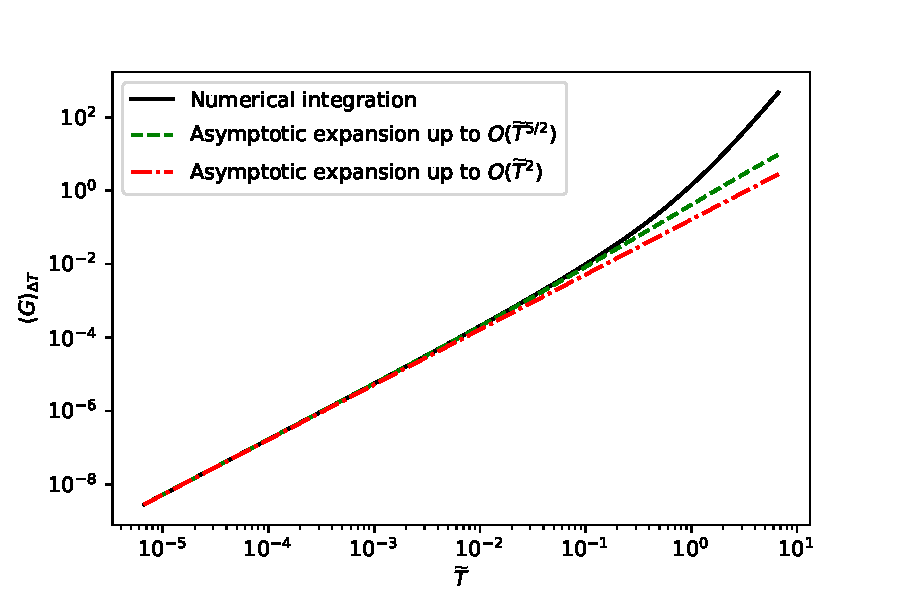
\includegraphics[width=0.49\textwidth]{./plot/expansion_comparison.pdf}
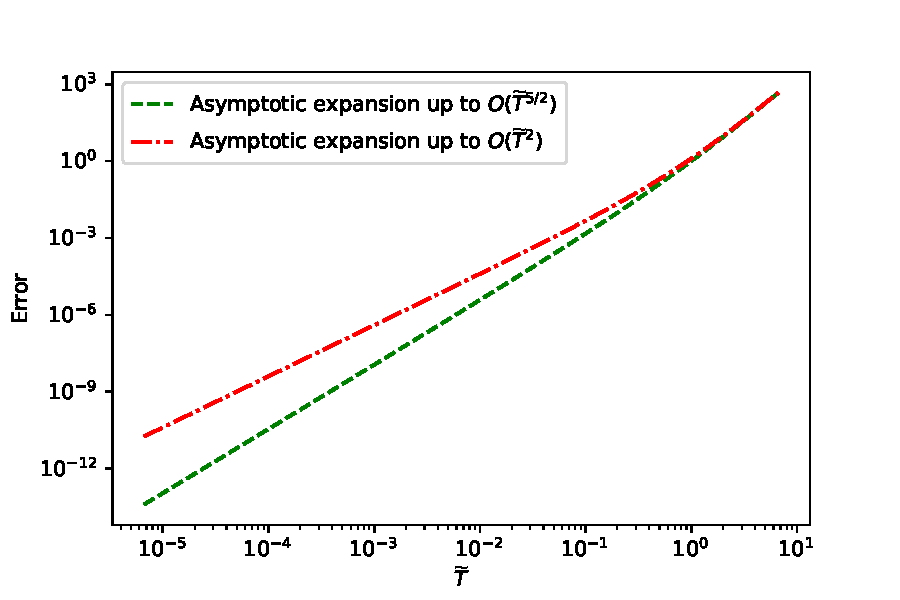
\includegraphics[width=0.49\textwidth]{./plot/expansion_error_comparison.pdf}
\caption{Comparison of the computation of $\langle G\rangle_{\Delta T}$ (left)   using the expansion \eqref{eq:expansion_b_decay} for $m=1.5$, $\gamma=1/2$, $B=1$, and $G(p)=(m+p)/E$ with the result obtained via numerical integration of \eqref{eq:b_decay_orig_integral}. The right plot shows the difference between the numerical result and the two expansions.  On a log-log plot they have slops of approximately $5/2$ and $2$, matching the indicated order of the expansion error in $\widetilde{T}$. }\label{fig:expansion_comparison}
\end{figure}




\begin{figure}
\centering
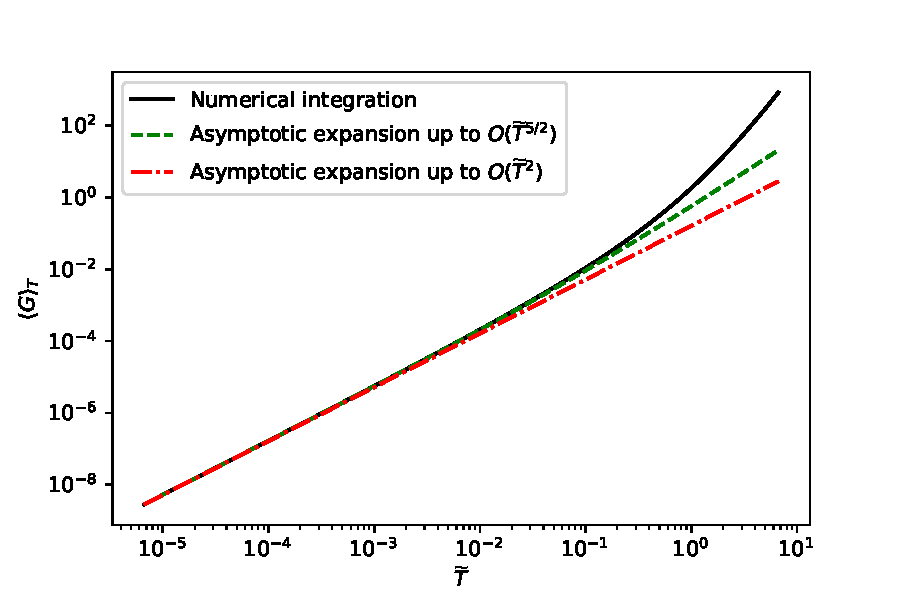
\includegraphics[width=0.49\textwidth]{./plot/FD_avg_expansion_comparison.pdf}
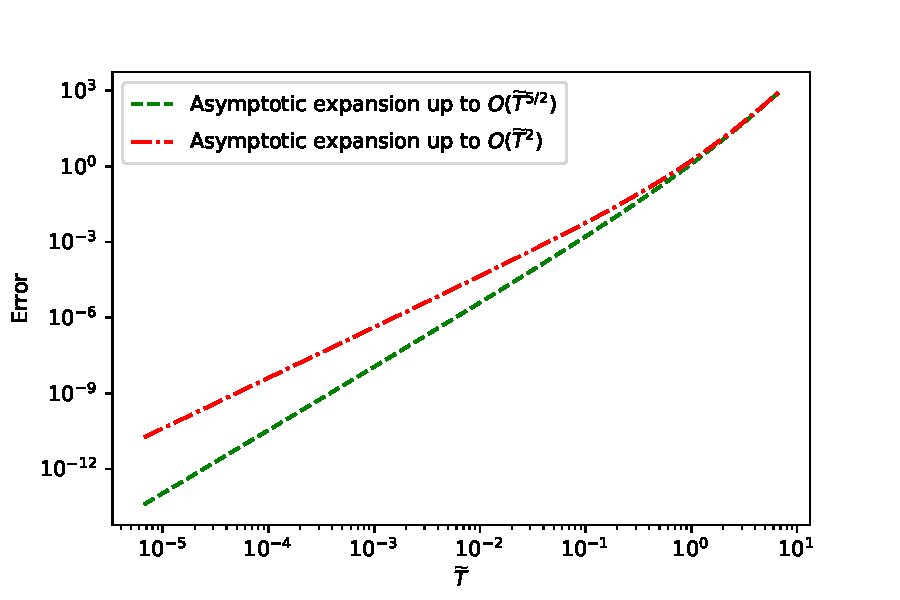
\includegraphics[width=0.49\textwidth]{./plot/FD_avg_expansion_error_comparison.pdf}
\caption{Comparison of the computation of $\langle G\rangle_{T}$ (left)   using the expansion \eqref{eq:asymp_FD_int_b_decay} for $D=3$, $m=1.5$, $\gamma=1/2$, $B=1$, and $G(p)=(m+p)/E$ with the result obtained via numerical integration of \eqref{eq:FD_b_decay_orig_integral}. The right plot shows the difference between the numerical result and the two expansions.  On a log-log plot  the slopes can be measured to be approximately $5/2$ and $2$, correctly matching the indicated order of the expansion error in $\widetilde{T}$. }\label{fig:FD_avg_expansion_comparison}
\end{figure}
